\documentclass[preprint,12pt]{elsarticle}

% --- Packages ---
\usepackage{amsmath,amssymb}
\usepackage{booktabs}
\usepackage{graphicx}
\usepackage{hyperref}
\usepackage{url}
\usepackage{xcolor}
\usepackage{lineno}
\usepackage{multirow}
\usepackage{siunitx}

% Enable line numbers for review
\modulolinenumbers[5]

% Figures are in figures/ subdirectory
\graphicspath{{figures/}}

\journal{Advances in Space Research}

\begin{document}

\begin{frontmatter}

\title{Economic Inflection Points in Space Manufacturing:\\ Monte Carlo Analysis of In-Situ Resource Utilization vs.\ Earth Launch for Large-Scale Space Infrastructure}

\author[dyson]{Thijs Hakkenberg\corref{cor1}}
\cortext[cor1]{Corresponding author.}
\ead{thijs@hakkenberg.com}
\fntext[fn1]{This research was conducted using an AI-assisted methodology. Claude (Anthropic), GPT (OpenAI), and Gemini (Google) were used for literature synthesis; editorial review and peer review simulation were conducted using all three models. The Monte Carlo simulation code was written and verified by the human author in Python using NumPy and SciPy. All quantitative results were produced by deterministic and stochastic simulation code; parameter ranges were informed by published literature and engineering analogy. No AI-generated numerical outputs were used without independent verification against the simulation code.}

\address[dyson]{Project Dyson, Open Research Initiative\fnref{fn1}}

\begin{abstract}
We present a parametric cost model comparing Earth-launch and in-situ resource utilization (ISRU) pathways for serial production of structural modules, incorporating NPV discounting, pathway-specific schedules, and Wright learning curves empirically supported in analogous programs for $n \leq 1{,}000$ units; extrapolation to higher volumes is tested via a piecewise plateau model. A 10{,}000-run Monte Carlo sampling fourteen independent stochastic parameters (plus two derived)---including log-normal ISRU capital calibrated to both Flyvbjerg terrestrial ($\sigma_{\ln} = 0.70$) and space-specific ($\sigma_{\ln} = 1.0$) reference classes---via a 3D Gaussian copula finds that for a program committing to 20{,}000 units, 42\% (95\% bootstrap CI: [41\%, 43\%]) of scenarios fall within the ISRU savings window at $r = 5\%$. The raw crossover probability is ${\sim}$69\% (within $H = 40{,}000$ units), decomposed into ${\sim}$6\% permanent and ${\sim}$63\% transient; the conditional median is ${\sim}5{,}000$~units. Rank-regression variance decomposition confirms that Earth learning rate and ISRU capital together explain ${\sim}70\%$ of output variance. Over 30 robustness tests---including product archetype sensitivity, $K$-clip bound analysis, and Earth-side scaling penalties---confirm crossover under diverse assumptions, though three factors can prevent it: vitamin component costs above ${\sim}\$50{,}000$/kg, discount rates above ${\sim}20\%$, or low technical success probability ($p_s \lesssim 70\%$). For revenue-generating infrastructure, the exact lost-revenue NPV of ISRU's deployment delay may offset savings at revenue rates above ${\sim}\$0.9$M/unit/yr, suggesting the ISRU advantage is strongest for non-revenue infrastructure.
\end{abstract}

\begin{keyword}
in-situ resource utilization \sep space manufacturing \sep launch cost \sep Monte Carlo simulation \sep learning curves \sep net present value \sep space economics
\end{keyword}

\end{frontmatter}

\linenumbers

%% ============================================================
\section{Introduction}
\label{sec:introduction}
%% ============================================================

Any program of large-scale space infrastructure construction---whether solar power satellites, orbital habitats, or distributed energy collection architectures---eventually reaches a decision point that no amount of launch cost reduction can fully avoid under Earth-supplied logistics: at what scale does it become cheaper to manufacture components in space rather than to build them on Earth and haul them up through the gravity well? At megascale, some fraction of each unit's mass must still be Earth-sourced (hereafter ``vitamin'' components, \S\ref{sec:vitamin}). This question has been posed qualitatively since at least the 1970s \cite{oneill1974,oneill1976}, and it has recently gained renewed urgency as launch costs decline precipitously \cite{jones2018}, lunar ISRU programs advance under the Artemis architecture \cite{sanders2015}, and private ventures pursue asteroid resource extraction \cite{elvis2012,andrews2015}.

The intuition is rooted in a cost asymmetry that launch cost reduction cannot fully eliminate. Reusable vehicles have brought per-kilogram costs down by roughly two orders of magnitude, from \$20{,}000/kg to projections below \$500/kg for Starship-class vehicles. But per-kilogram launch costs decline more slowly than manufacturing costs: even under aggressive launch learning (LR$_L = 0.90$), the propellant and operations component ($\sim$\$200/kg) constitutes an assumed operational asymptote under Earth-supplied logistics that the learnable component cannot breach. ISRU inverts this cost structure: large fixed capital costs up front, but each additional unit produced from local materials costs only energy and labor. The fixed costs divide across a growing denominator; marginal costs decline with experience.

Despite the intuitive appeal of this argument, a quantitative gap persists in the literature. Existing ISRU economic analyses are overwhelmingly mission-specific: they evaluate the cost-effectiveness of producing lunar oxygen for propellant \cite{sanders2015}, extracting water ice for life support \cite{zubrin1996}, or mining asteroidal platinum-group metals for terrestrial markets \cite{sonter1997,elvis2012}. We are not aware of prior work that combines schedule-aware NPV crossover analysis with systematic uncertainty characterization for generic manufactured products.

A second gap concerns the treatment of manufacturing learning. The Wright learning curve \cite{wright1936}, well established in aerospace production economics \cite{wertz2011}, predicts that unit manufacturing cost decreases as a power function of cumulative production volume. This effect has been extensively documented for Earth-based aerospace systems \cite{argote1990,nagy2013} but we are not aware of it being combined with NPV timing analysis in a comparative Earth-versus-ISRU cost model for generic structural units. The omission matters because the two pathways exhibit fundamentally different learning dynamics: Earth manufacturing benefits from learning in fabrication but exhibits limited learning in launch (baseline $\mathrm{LR}_L = 0.97$; we sweep from 90\% to 100\% in \S\ref{sec:sensitivity}), while ISRU benefits from learning in both extraction and fabrication, albeit from a higher initial cost base and with a slower initial ramp-up. The long-run consequences of this asymmetry are not obvious without a quantitative model.

Our analysis is primarily relevant to non-revenue infrastructure (habitats, depots, structural frameworks) where cost minimization is the decision criterion. For revenue-generating systems such as space solar power, the opportunity cost of ISRU's deployment delay may dominate the cost savings (\S\ref{sec:discussion}), making the Earth pathway preferred even above the cost crossover.

This paper makes three contributions. First, we present a parametric cost model with net present value discounting and pathway-specific delivery schedules that expresses the total cost of producing $N$ units via the Earth-launch pathway and the ISRU pathway as explicit functions of production volume, with learning curves, an integrated production ramp-up schedule, ISRU mass penalty and transport costs, and financing costs applied to the appropriate components (\S\ref{sec:model}). Second, we embed this model in a 10{,}000-run Monte Carlo framework with correlated sampling that propagates uncertainty in fourteen independent stochastic parameters (plus two derived)---including the ISRU operational cost floor, production rate, and transport duration---at each of several fixed discount rates, yielding probability distributions, convergence analysis, and global sensitivity rankings rather than point estimates (\S\ref{sec:results}). Third, we propose a phased hybrid transition strategy and discuss its implications for near-term space policy (\S\ref{sec:discussion}).

%% ============================================================
\section{Related Work}
\label{sec:related}
%% ============================================================

The economic case for ISRU has been examined primarily for mission-specific applications. Sanders and Larson \cite{sanders2015} found lunar oxygen extraction cost-effective after approximately five crewed missions, but their model does not generalize to manufactured goods. Crawford \cite{crawford2015} catalogued lunar mineralogical inventories; Cilliers et al.\ \cite{cilliers2023} examined regolith processing pathways; Kornuta et al.\ \cite{kornuta2019} developed a commercial lunar propellant architecture. The MOXIE experiment \cite{hecht2021} provided empirical validation of in-situ oxygen production on Mars, though at sub-manufacturing scales. Sowers \cite{sowers2021,sowers2023} presented NPV-based business cases for lunar ice mining and cislunar economics. Metzger et al.\ \cite{metzger2013} proposed a bootstrapping approach in which a seed factory progressively builds its own capacity. Asteroid mining NPV frameworks have been developed by Sonter \cite{sonter1997}, Elvis \cite{elvis2012}, and Andrews et al.\ \cite{andrews2015}; Ishimatsu et al.\ \cite{ishimatsu2016} modeled Earth--Moon--Mars logistics as a multicommodity network flow. These analyses focus on resource extraction rather than structural manufacturing. Lunar additive manufacturing demonstrations \cite{werkheiser2015,cesaretti2014} provide empirical grounding for the ISRU manufacturing pathway assumed here. O'Neill \cite{oneill1974,oneill1976} argued on energetic grounds for lunar material delivery to orbit, but lacked a parametric cost model and did not incorporate learning curves. The real options framework \cite{dixit1994} extends NPV for irreversible investments under uncertainty; Saleh et al.\ \cite{saleh2003} applied flexibility analysis to spacecraft, and de~Weck et al.\ \cite{deweck2004} demonstrated staged deployment value. Organizational forgetting \cite{benkard2000,thompson2012} has been documented in aerospace production lines.

Jones \cite{jones2018,jones2020,jones2022} documented a roughly two-orders-of-magnitude reduction in launch cost per kilogram over six decades. A critical distinction is between vehicle manufacturing cost (which follows a learning curve) and per-kilogram delivery cost (dominated by propellant and operations, largely independent of cumulative launches). Falcon~9 reuse economics \cite{zapata2019} confirm that per-launch cost reductions arise from fixed-cost amortization at high flight rates, not production learning. Wertz \cite{wertz2011} estimated launch vehicle production learning rates of 85--90\%; the NASA Cost Estimating Handbook \cite{nasa2015handbook} provides standardized parametric methodologies that inform our parameter selection. Our model adopts a two-component launch cost: a propellant operational asymptote plus a learnable component ($\mathrm{LR}_L = 0.97$); we sweep $\mathrm{LR}_L$ from 0.90 to 1.00 in \S\ref{sec:sensitivity}.

The Wright learning curve \cite{wright1936}---in which unit cost decreases as a power function of cumulative production---is well established in aerospace economics \cite{dutton1984,argote1990,nagy2013}; we formalize it in \S\ref{sec:model} (Eq.~\ref{eq:earth_mfg}). Typical aerospace learning rates range from 0.80 to 0.95 \cite{wertz2011}; Baumers et al.\ \cite{baumers2016} documented 0.85--0.92 for metal additive manufacturing. We are not aware of prior work applying the Wright model to a comparative Earth-versus-ISRU manufacturing analysis with NPV timing.

%% ============================================================
\section{Model Description}
\label{sec:model}
%% ============================================================

\paragraph{Decision problem.} The primary comparison metric is the NPV of cumulative cost to deliver the first $N$ units (Eq.~\ref{eq:crossover_npv}), where each pathway delivers according to its own schedule. This answers: ``Given a program requirement of $N$ structural modules, which pathway has lower total present-value cost?'' Section~\ref{sec:discussion} extends this to a utility-maximizing framing (Eq.~\ref{eq:revenue_breakeven}) that accounts for revenue per unit and the opportunity cost of ISRU's deployment delay.

We model the total cost of producing $N$ identical structural modules (hereafter ``units'') via two pathways: an Earth-launch pathway and an ISRU pathway. Each unit has a reference mass $m = 1{,}850$~kg, representative of structural modules in the 1{,}000--5{,}000~kg class typical of solar collector or orbital habitat components, though the model is parameterizable to other mass ranges. We describe each pathway's cost model, then the Monte Carlo framework used to propagate parameter uncertainty.

\paragraph{Reference orbit.} Throughout this paper, ``operational orbit'' refers to geostationary Earth orbit (GEO), consistent with space solar power and communications relay architectures. The launch cost $p_{\mathrm{launch}}$ represents delivery from Earth surface to GEO; the transport cost $p_{\mathrm{transport}}$ represents delivery from the lunar surface to GEO via low-energy trajectory ($\sim$6~km/s $\Delta v$). For other destinations (LEO, NRHO, cislunar), both cost terms would differ; the model is parameterizable to any orbit.

\paragraph{Cost basis normalization.} All launch costs in this paper are quoted for delivery to GEO. Published Starship cost projections (\$200--500/kg) typically refer to LEO; delivery to GEO via an upper stage or electric tug adds a factor of $\sim$2--3$\times$, so \$500/kg to LEO corresponds to approximately \$1,000--1,500/kg to GEO, consistent with our baseline of \$1,000/kg. The operational asymptote $p_{\mathrm{fuel}}$ is now sampled stochastically: $p_{\mathrm{fuel}} \sim U[\$100, \$400]$/kg (baseline \$200/kg). A bottom-up decomposition of the GEO delivery cost chain (propellant, LEO-to-GEO transfer, ground operations; Appendix~\ref{sec:appendix_params}) yields a total floor of $\sim$\$105--178/kg, with \$200/kg as the central estimate; the $U[\$100, \$400]$ range brackets optimistic and conservative assumptions.

\subsection{Earth-launch pathway}

The cost of the $n$th unit produced on Earth and launched to the operational orbit is
\begin{equation}
  C_{\mathrm{Earth}}(n) = C_{\mathrm{mfg}}(n) + C_{\mathrm{launch}}(n),
  \label{eq:earth_unit}
\end{equation}
where $C_{\mathrm{mfg}}(n)$ is the terrestrial manufacturing cost and $C_{\mathrm{launch}}(n)$ is the launch cost. Manufacturing cost follows a two-component model separating non-learnable material costs from learnable labor and overhead:
\begin{equation}
  C_{\mathrm{mfg}}(n) = C_{\mathrm{mat}} + C_{\mathrm{labor}}^{(1)} \cdot n^{\,b_E}, \quad b_E = \frac{\ln(\mathrm{LR}_E)}{\ln 2},
  \label{eq:earth_mfg}
\end{equation}
where $C_{\mathrm{mat}} = \$1$M is the per-unit material cost in constant 2024 real dollars (aerospace-grade structural materials at $\sim$\$540/kg $\times$ 1{,}850~kg $\approx$ \$1M), which does not decline with cumulative production, and $C_{\mathrm{labor}}^{(1)} = \$74$M is the first-unit recurring cost (labor, overhead, and amortized tooling/NRE spread across the first production lot---not a separate fixed charge), which follows the Wright learning curve with Earth learning rate $\mathrm{LR}_E$. Note: a \emph{higher} learning rate (closer to 1.0) means \emph{slower} learning; $\mathrm{LR}_E = 0.85$ implies a 15\% cost reduction per doubling of cumulative production. The first-unit total is $C_{\mathrm{mfg}}^{(1)} = C_{\mathrm{mat}} + C_{\mathrm{labor}}^{(1)} = \$1\text{M} + \$74\text{M} = \$75\text{M}$. The material cost serves as a natural manufacturing cost floor---more physically motivated than an arbitrary floor parameter---because no amount of production learning eliminates the cost of raw materials. At $n = 10{,}000$, the labor component has declined to $\sim$\$7.2M while the material cost remains \$1M, yielding a total of $\sim$\$8.2M---compared to $\sim$\$8.2M under the single Wright curve. The two-component model produces nearly identical crossover results at baseline but provides a clearer physical interpretation: the floor is material cost, not an arbitrary truncation. For backward compatibility, we retain a manufacturing cost floor parameter $C_{\mathrm{mfg}}^{\mathrm{floor}}$ that can be applied on top of the two-component model; the baseline uses $C_{\mathrm{mfg}}^{\mathrm{floor}} = 0$.
\begin{equation}
  C_{\mathrm{mfg}}(n) = \max\!\left(C_{\mathrm{mat}} + C_{\mathrm{labor}}^{(1)} \cdot n^{\,b_E},\; C_{\mathrm{mfg}}^{\mathrm{floor}}\right).
  \label{eq:earth_mfg_floor}
\end{equation}
As a reference case, launch cost can be treated as constant when the program's launch demand is a small fraction of total market demand:
\begin{equation}
  C_{\mathrm{launch}}(n) = m \cdot p_{\mathrm{launch}},
  \label{eq:earth_launch_baseline}
\end{equation}
i.e., a constant \$1{,}000/kg $\times$ 1{,}850~kg $=$ \$1.85M per unit. The baseline MC instead uses a two-component model with program-indexed learning:
\begin{equation}
  C_{\mathrm{launch}}^{\mathrm{learn}}(n) = m \left[ p_{\mathrm{fuel}} + p_{\mathrm{ops}} \cdot n^{\,b_L} \right], \quad b_L = \frac{\ln(\mathrm{LR}_L)}{\ln 2},
  \label{eq:earth_launch_learn}
\end{equation}
where $p_{\mathrm{fuel}} = \$200$/kg is an assumed operational asymptote under Earth-supplied propellant logistics (propellant plus minimal GEO delivery operations) and $p_{\mathrm{ops}} = \$800$/kg is the learnable component, declining at $\mathrm{LR}_L = 0.97$ per doubling (see Table~\ref{tab:config}).

In the Monte Carlo, $p_{\mathrm{launch}}$ is sampled from $U[500, 2000]$ and $p_{\mathrm{fuel}}$ from $U[100, 400]$. The learnable component is derived as $p_{\mathrm{ops}} = \max(p_{\mathrm{launch}} - p_{\mathrm{fuel}}, 0)$, ensuring the total first-unit launch cost equals the sampled $p_{\mathrm{launch}}$ while the operational asymptote matches $p_{\mathrm{fuel}}$.

For the deterministic baseline, the two formulations yield practically identical results: at baseline scale (${\sim}4{,}400$~units), the ops component under $\mathrm{LR}_L = 0.97$ declines by less than 0.3\%, a shift smaller than the search grid resolution (Table~\ref{tab:launch_learning}). We sweep $\mathrm{LR}_L$ from 0.90 to 1.00 in \S\ref{sec:sensitivity}; even at aggressive learning the crossover shifts by only $+$315~units ($+$7\%), confirming that the model's conclusions are insensitive to the launch learning assumption.

\textbf{Indexing convention.} The learning index $n$ counts cumulative program units. At the assumed program scale ($\sim$4{,}100--10{,}000 units), the program would constitute a substantial fraction of global launch demand, making program-indexed learning a reasonable proxy for market-indexed learning.

The cumulative cost of producing $N$ units via the Earth pathway is therefore
\begin{equation}
  \Sigma_{\mathrm{Earth}}(N) = \sum_{n=1}^{N} \left[ \max\!\left(C_{\mathrm{mat}} + C_{\mathrm{labor}}^{(1)} \cdot n^{\,b_E},\; C_{\mathrm{mfg}}^{\mathrm{floor}}\right) + m \cdot p_{\mathrm{launch}} \right].
  \label{eq:earth_cum}
\end{equation}
When the launch learning sensitivity variant (Eq.~\ref{eq:earth_launch_learn}) is active, $m \cdot p_{\mathrm{launch}}$ is replaced by the two-component expression.

\subsection{ISRU pathway}

\subsubsection{Production schedule and ramp-up}

A critical distinction between the two pathways is their delivery timing. Earth manufacturing can begin immediately upon program start, requiring no new infrastructure beyond existing terrestrial supply chains. The ISRU pathway, by contrast, requires construction and commissioning of an extraterrestrial facility before production can begin, followed by a logistic ramp-up to full capacity.

\paragraph{Earth delivery schedule.} The Earth pathway delivers units at a constant rate from $t = 0$:
\begin{equation}
  t_{n,E} = \frac{n}{\dot{n}_{\max}},
  \label{eq:earth_schedule}
\end{equation}
where $\dot{n}_{\max}$ is the full-capacity production rate (units/year). This assumes pre-existing Earth manufacturing capacity, reasonable given the maturity of terrestrial aerospace production; we test a logistic Earth ramp-up ($t_{0,E} \in \{1, 2\}$~yr) in \S\ref{sec:earth_ramp}.

\paragraph{ISRU delivery schedule.} The ISRU facility's instantaneous production rate follows a logistic ramp-up function:
\begin{equation}
  \dot{n}(t) = \dot{n}_{\max} \cdot S(t), \quad S(t) = \frac{1}{1 + e^{-k(t - t_0)}},
  \label{eq:scurve}
\end{equation}
where $t_0$ is the ramp-up midpoint (years from program start) and $k = 2.0$ (fixed) controls steepness. Integrating the production rate yields the cumulative production function:
\begin{equation}
  N(t) = \frac{\dot{n}_{\max}}{k} \left[ \ln\!\left(1 + e^{k(t - t_0)}\right) - \ln 2 \right],
  \label{eq:cumulative_production}
\end{equation}
The constant $-\ln 2$ ensures $N(t_0) = 0$. A piecewise formulation enforces $\dot{n}(t) = 0$ for $t < t_c$ ($t_c = t_0 - 1$ by default); at $t = t_0$ the rate is half-maximal, exceeding 90\% capacity within ${\sim}1$~year (Figure~\ref{fig:production_schedule}). The closed-form inverse gives the calendar time of the $n$th ISRU unit:
\begin{equation}
  t_{n,I} = t_0 + \frac{1}{k} \ln\!\left(2\,e^{nk/\dot{n}_{\max,\mathrm{eff}}} - 1\right).
  \label{eq:production_schedule}
\end{equation}
(obtained by inverting Eq.~\ref{eq:cumulative_production}). Note that $t_{n,I}$ includes the pre-production construction period: $t_0$ encompasses both facility construction and commissioning (Eqs.~\ref{eq:scurve}--\ref{eq:cumulative_production}).

We introduce a transport duration $\tau_{\mathrm{trans}}$ (baseline 0.5~yr) representing low-energy lunar-to-GEO transfer, so delivery time is
\begin{equation}
  t_{n,I}^{\mathrm{del}} = t_{n,I} + \tau_{\mathrm{trans}}.
  \label{eq:delivery_time}
\end{equation}
Discounting and revenue-delay calculations use the delivery time $t_{n,I}^{\mathrm{del}}$ rather than the production time $t_{n,I}$. In the Monte Carlo, $\tau_{\mathrm{trans}} \sim U[0.25, 2.0]$~yr, bracketing chemical ($\sim$0.25~yr) and solar-electric ($\sim$1$-$2~yr) low-energy transfer options.

The effective ISRU production rate accounts for facility availability:
\begin{equation}
  \dot{n}_{\max,\mathrm{eff}} = A \cdot \dot{n}_{\max},
  \label{eq:availability}
\end{equation}
where $A \in [0,1]$ is the fraction of calendar time the facility is operational. The deterministic baseline uses $A = 1.0$ (backward-compatible); the Monte Carlo samples $A \sim U[0.70, 0.95]$.

\paragraph{Timing gap.} The separation between these schedules is substantial: when Earth has delivered its 1{,}000th unit ($t = 2$~yr), ISRU has not yet produced any (its 1{,}000th unit arrives at $t \approx 7.3$~yr; Table~\ref{tab:production_schedule} in Appendix~\ref{sec:appendix_schedule}). This gap has a counterintuitive NPV consequence: because Earth costs are incurred earlier, they are discounted \emph{less}, making the Earth pathway more expensive in NPV terms. This partially offsets the ISRU pathway's heavy upfront capital burden.

\subsubsection{Cost model}

For illustrative comparison of per-unit costs, the ISRU Average Unit Cost (AUC) of the $n$th unit can be expressed as an amortized capital component plus an operational component:
\begin{equation}
  C_{\mathrm{ISRU}}^{\mathrm{AUC}}(n) = \frac{K}{N_{\mathrm{total}}} + C_{\mathrm{ops}}(n),
  \label{eq:isru_unit}
\end{equation}
where $K$ is the total capital investment required to establish the ISRU infrastructure, and $N_{\mathrm{total}}$ is a planning horizon over which capital is amortized for display purposes. We set $N_{\mathrm{total}} = 10{,}000$ throughout; this choice affects the per-unit cost visualization (Figure~\ref{fig:unitcost}) but does not enter the crossover calculation, which uses the cumulative formulation below.

The operational cost follows a Wright learning curve with a cost floor $C_{\mathrm{floor}}$ representing irreducible per-unit expenses (energy, consumables, remote operations overhead), scaled by a mass penalty factor $\alpha$ and augmented by a transport cost for delivering ISRU-manufactured units to the operational orbit:
\begin{equation}
  C_{\mathrm{ops}}(n) = \alpha \left[ C_{\mathrm{floor}} + \left(C_{\mathrm{ops}}^{(1)} - C_{\mathrm{floor}}\right) \cdot n^{\,b_I} \right] + m \cdot p_{\mathrm{transport}} \cdot \alpha,
  \label{eq:isru_ops}
\end{equation}
where $b_I = \ln(\mathrm{LR}_I)/\ln 2$ with ISRU learning rate $\mathrm{LR}_I$, $C_{\mathrm{floor}}$ represents the asymptotic minimum operational cost per unit (energy, consumables, remote operations overhead), $\alpha \geq 1$ is a delivered-mass penalty: an ISRU-manufactured unit with $\alpha = 1.3$ has 30\% more mass than the reference design (thicker structural margins, lower-purity alloys) and therefore requires proportionally more processing and transport---both operational cost and transport cost scale with $\alpha$ because both are proportional to the mass actually processed and delivered---and $p_{\mathrm{transport}}$ (\$/kg) is the cost of transporting an ISRU-manufactured unit from the production site to the operational orbit. The cost floor is sampled as $C_{\mathrm{floor}} \sim U[\$0.3\text{M}, \$2.0\text{M}]$ in the Monte Carlo; when $C_{\mathrm{floor}}$ exceeds the Earth pathway's per-unit launch cost floor ($m \cdot p_{\mathrm{launch}} = \$1.85$M at baseline), the per-unit cost advantage of ISRU is reduced, potentially preventing crossover within the planning horizon. This scenario is captured in the non-convergence statistics (\S\ref{sec:mc_robustness}).

The ramp-up effect is captured purely through timing: early units are produced later and therefore discounted more heavily in the NPV calculation (Eq.~\ref{eq:production_schedule}). The cumulative cost of producing $N$ units via the ISRU pathway is
\begin{equation}
  \Sigma_{\mathrm{ISRU}}(N) = K + \sum_{n=1}^{N} C_{\mathrm{ops}}(n).
  \label{eq:isru_cum}
\end{equation}
Note that the full capital cost $K$ is incurred upfront; the amortized per-unit formulation (Eq.~\ref{eq:isru_unit}) is used only for visualization.

\subsubsection{Crossover and NPV formulation}

The undiscounted crossover $N^*_0$ is the smallest $N$ with $\Sigma_{\mathrm{ISRU}}(N) \leq \Sigma_{\mathrm{Earth}}(N)$. Because the ISRU pathway concentrates expenditure early while Earth distributes costs over time, each pathway's costs must be discounted according to its own delivery schedule. We define the NPV crossover $N^*$ as the smallest $N$ satisfying
\begin{equation}
  K + \sum_{n=1}^{N} \frac{C_{\mathrm{ops}}(n)}{(1+r)^{t_{n,I}^{\mathrm{del}}}} \;\leq\; \sum_{n=1}^{N} \frac{C_{\mathrm{Earth}}(n)}{(1+r)^{t_{n,E}}},
  \label{eq:crossover_npv}
\end{equation}
where $r$ is the real discount rate (all costs in constant 2024 USD) and $t_{n,I}^{\mathrm{del}} = t_{n,I} + \tau_{\mathrm{transport}}$ is the ISRU delivery time including transport from the production site to the operational orbit (the code has always discounted at delivery time; this notation makes the convention explicit). In the baseline formulation, $K$ is incurred at $t = 0$; in the phased formulation (\S\ref{sec:phased_capital}), $K$ is spread over five annual tranches. Because Earth costs are incurred earlier ($t_{n,E} < t_{n,I}^{\mathrm{del}}$), they carry higher present value, making the Earth pathway more expensive in NPV terms; this partially offsets the ISRU pathway's upfront capital burden. When $r = 0$, Eq.~\ref{eq:crossover_npv} reduces to the undiscounted comparison.

\paragraph{Permanent vs.\ transient crossover classification.} A crossover is \emph{permanent} if the ISRU pathway remains cheaper at all subsequent production volumes, and \emph{transient} if the Earth pathway eventually re-crosses at very large $n$. Formally, the crossover is permanent iff
\begin{equation}
  \lim_{n \to \infty} C_{\mathrm{ISRU}}^{\mathrm{ops}}(n) \;<\; \lim_{n \to \infty} C_{\mathrm{Earth}}(n).
  \label{eq:permanent}
\end{equation}
The ISRU asymptotic per-unit cost (learning terms $\to$ 0) is
\[
  C_{\mathrm{ISRU}}^{\infty} = (1 - f_v)\bigl[\alpha \, C_{\mathrm{floor}} + m \, p_{\mathrm{transport}} \, \alpha\bigr] + f_v \, m \bigl(p_{\mathrm{fuel}} + c_{\mathrm{vit}}\bigr),
\]
and the Earth asymptotic per-unit cost is
\[
  C_{\mathrm{Earth}}^{\infty} = C_{\mathrm{mat}} + m \, p_{\mathrm{fuel}},
\]
where the learnable components ($C_{\mathrm{labor}}$, $p_{\mathrm{ops}}$) vanish at large $n$. When $f_v > 0$, the vitamin component contributes a non-vanishing term ($f_v \cdot m \cdot c_{\mathrm{vit}} \approx \$0.93$M at baseline), which can raise $C_{\mathrm{ISRU}}^{\infty}$ above $C_{\mathrm{Earth}}^{\infty}$, making most crossovers transient. The Monte Carlo classifies each run using Eq.~\ref{eq:permanent}; see \S\ref{sec:mc_robustness} for results.

For transient crossovers, we define the \emph{re-crossing volume} $N^{**}$ as the smallest $N > N^*$ at which the ISRU cumulative NPV cost again exceeds the Earth pathway:
\begin{equation}
  N^{**} = \min\!\left\{N > N^* \;:\; \sum_{n=1}^{N} \frac{C_{\mathrm{ops}}(n)}{(1+r)^{t_{n,I}^{\mathrm{del}}}} + K \;>\; \sum_{n=1}^{N} \frac{C_{\mathrm{Earth}}(n)}{(1+r)^{t_{n,E}}}\right\}.
  \label{eq:recrossing}
\end{equation}
$N^{**}$ is searched up to $N = 200{,}000$; runs that do not re-cross within this bound are right-censored.\footnote{With NPV discounting, late-arriving costs are heavily attenuated, so many asymptotically transient scenarios do not re-cross within any practical horizon.} The savings window $[N^*, N^{**}]$ represents the production range over which ISRU is cost-advantaged. We distinguish three categories based on this framework:
\begin{itemize}
\item \textbf{Asymptotically permanent} (Eq.~\ref{eq:permanent}): $C_{\mathrm{ISRU}}^{\infty} < C_{\mathrm{Earth}}^{\infty}$; ISRU per-unit cost is lower at $n \to \infty$.
\item \textbf{Finite-horizon permanent}: $N^{**} > 200{,}000$; does not re-cross within the search bound despite $C_{\mathrm{ISRU}}^{\infty} \geq C_{\mathrm{Earth}}^{\infty}$.
\item \textbf{Finite-horizon transient}: $N^{**} \leq 200{,}000$; re-crosses within the search bound.
\end{itemize}

\subsubsection{Earth-sourced component fraction}
\label{sec:vitamin}

Even passive structural modules require Earth-sourced fasteners, seals, sensors, and coatings. We model this via a vitamin fraction $f_v$: a fraction $f_v$ of each unit's mass must be launched from Earth, with its own manufacturing cost $c_{\mathrm{vit}}$ (\$/kg). The ISRU operational cost becomes
\begin{equation}
  C_{\mathrm{ops}}^{\mathrm{vit}}(n) = (1 - f_v) \cdot C_{\mathrm{ops}}(n) + f_v \cdot m \cdot \bigl(p_{\mathrm{launch,eff}}(n) + c_{\mathrm{vit}}\bigr),
  \label{eq:vitamin}
\end{equation}
where $p_{\mathrm{launch,eff}}(n)$ includes launch learning when active (i.e., the Earth pathway's two-component model, Eq.~\ref{eq:earth_launch_learn}), and $c_{\mathrm{vit}} = \$10{,}000$/kg reflects the manufacturing cost of mechanical vitamin components---fasteners, seals, coatings, and simple sensors---rather than radiation-hardened electronics (which can exceed \$100{,}000/kg \cite{wertz2011}). The \$10{,}000/kg figure is grounded in specialty aerospace mechanical components at volumes of 100--1{,}000 units; the sensitivity analysis tests $c_{\mathrm{vit}} = \$50{,}000$/kg to bound the case where rad-hard electronics are included in the vitamin fraction. The baseline uses $f_v = 0.05$ (5\% of unit mass Earth-sourced). This vitamin fraction is included in the baseline because it drives the permanent/transient crossover distinction (\S\ref{sec:mc_robustness}): at large $n$, the vitamin component's asymptotic cost ($f_v \cdot m \cdot (p_{\mathrm{fuel}} + c_{\mathrm{vit}}) \approx \$0.94$M) raises the ISRU floor above the Earth pathway's asymptotic cost, making most crossovers transient (finite-horizon amortization effects). This is a conservative modeling choice; if vitamin components can eventually be ISRU-sourced, all crossovers become permanent. The $f_v = 0$ case (fully ISRU-derived, an optimistic bound) is reported as a sensitivity variant. We test $f_v \in \{0, 0.05, 0.10, 0.15, 0.20\}$ and $c_{\mathrm{vit}} \in \{\$5{,}000, \$10{,}000, \$50{,}000\}$/kg in \S\ref{sec:sensitivity}. A deterministic sweep of $f_v$ from 0 to 0.20 (at 1\% increments) reveals a permanence cliff: the transition from permanent to transient crossover occurs at $f_v \approx 4\%$, corresponding to the point where the vitamin component raises $C_{\mathrm{ISRU}}^{\infty}$ above $C_{\mathrm{Earth}}^{\infty}$. Below this threshold, all crossovers are permanent; above it, crossovers remain achievable but are finite-horizon amortization effects---though in practice $f_v$ would likely decrease at very large $N$ as ISRU capabilities mature, converting transient crossovers to permanent (\S\ref{sec:discussion}).

A representative mass breakdown (Table~\ref{tab:vitamin_bom} in Appendix~\ref{sec:appendix_params}) connects the 15\% total vitamin content to the 5\% irreducible Earth-sourced fraction.

\subsection{Monte Carlo framework}

To characterize the sensitivity of $N^*$ to parameter uncertainty, we embed the NPV cost model in a Monte Carlo simulation. Each of 10{,}000~runs samples fourteen independent parameter values (plus two derived) from the distributions specified in Table~\ref{tab:params} and computes the NPV crossover point via Eq.~\ref{eq:crossover_npv}. We define ``crossover achievement within horizon $H$'' (also referred to as ``convergence'' in tables) as the event $N^* \leq H$; throughout this paper, $H = 40{,}000$ unless otherwise stated. Critically, the discount rate $r$ is \emph{not} treated as a stochastic parameter. Instead, the full Monte Carlo ensemble is run independently at each of several fixed discount rates ($r \in \{3\%, 5\%, 8\%\}$). This separation is motivated by the observation that the discount rate reflects the decision-maker's time preference and financing structure rather than technological uncertainty; conflating it with stochastic cost parameters obscures the distinct roles of economic policy and engineering risk \cite{arrow2014}. We report the median, interquartile range, and 10th/90th percentiles of the resulting crossover distribution at each rate, with 95\% bootstrap confidence intervals computed from 5{,}000 bootstrap resamples.

\begin{table}[htbp]
\centering
\caption{Monte Carlo parameter distributions. Launch cost, ISRU capital, and production rate are correlated via a 3D Gaussian copula ($\rho_{p,K} = 0.3$, $\rho_{K,\dot{n}} = 0.5$); all other parameters are sampled independently. ISRU capital follows a log-normal distribution; results are presented at dual baselines $\sigma_{\ln} = 0.70$ (Flyvbjerg terrestrial, P90/P50 $\approx 2.5\times$) and $\sigma_{\ln} = 1.0$ (space-specific, P90/P50 $\approx 4.1\times$). The Monte Carlo is run at fixed discount rates $r \in \{3\%, 5\%, 8\%\}$. Achieving crossover is defined as $N^* \leq H$ where $H = 40{,}000$. Baseline values are rounded for exposition; the simulation uses exact values as specified in the code repository.}
\label{tab:params}
\resizebox{\textwidth}{!}{%
\begin{tabular}{@{}llll@{}}
\toprule
Parameter & Baseline & Distribution & Range \\
\midrule
\multicolumn{4}{@{}l}{\emph{Stochastic parameters (14 independent + 2 derived = 16 total)$^{\P}$}} \\
Launch cost $p_{\mathrm{launch}}$ (\$/kg) & 1{,}000 & Uniform$^\dagger$ & [500, 2{,}000] \\
ISRU capital $K$ (\$B) & 50 & Log-normal$^\dagger$ & med.\ 65, $\sigma_{\ln}$=0.70, clip [20, 200] \\
Earth learning rate $\mathrm{LR}_E$ & 0.85 & $\mathcal{N}(0.85, 0.03)$ & [0.75, 0.95] \\
ISRU learning rate $\mathrm{LR}_I$ & 0.90 & $\mathcal{N}(0.90, 0.03)$ & [0.80, 0.98] \\
Ramp-up time $t_0$ (years) & 5 & Uniform & [3, 8] \\
First-unit ops.\ cost $C_{\mathrm{ops}}^{(1)}$ (\$M) & 5 & Uniform & [2, 10] \\
First-unit mfg.\ cost $C_{\mathrm{mfg}}^{(1)}$ (\$M) & 75 & Uniform & [50, 100] \\
\quad Material cost $C_{\mathrm{mat}}$ (\$M) & 1.0 & Uniform & [0.5, 2.0] \\
\quad Labor cost $C_{\mathrm{labor}}^{(1)}$ (\$M) & 74$^\S$ & Derived & $C_{\mathrm{mfg}}^{(1)} - C_{\mathrm{mat}}$ \\
Mass penalty $\alpha$ & 1.0 & Uniform & [1.0, 2.0] \\
Transport cost $p_{\mathrm{transport}}$ (\$/kg) & 100 & Uniform & [50, 300] \\
Ops cost floor $C_{\mathrm{floor}}$ (\$M) & 0.5 & Uniform & [0.3, 2.0] \\
Production rate $\dot{n}_{\max}$ (units/yr) & 500 & Uniform & [250, 750] \\
ISRU availability $A$ & $1.0^\ddagger$ & Uniform & [0.70, 0.95] \\
Launch cost floor $p_{\mathrm{fuel}}$ (\$/kg) & 200 & Uniform & [100, 400] \\
Learnable launch comp.\ $p_{\mathrm{ops}}$ (\$/kg) & 800$^{\|}$ & Derived & $\max(p_{\mathrm{launch}} - p_{\mathrm{fuel}}, 0)$ \\
Transport duration $\tau_{\mathrm{trans}}$ (yr) & 0.5 & Uniform & [0.25, 2.0] \\
\midrule
\multicolumn{4}{@{}l}{\emph{Fixed parameters}} \\
Discount rate $r$ & 0.05 & Fixed per run & $\{0.03, 0.05, 0.08\}$ \\
Unit mass $m$ (kg) & 1{,}850 & Fixed & --- \\
S-curve steepness $k$ & 2.0 & Fixed & --- \\
Amortization horizon $N_{\mathrm{total}}$ & 10{,}000 & Fixed & --- \\
Launch--capital correlation $\rho_{p,K}$ & 0.3 & Fixed & --- \\
Capital--production rate corr.\ $\rho_{K,\dot{n}}$ & 0.5 & Fixed & --- \\
\bottomrule
\multicolumn{4}{@{}l}{\footnotesize $^\dagger$Launch cost and capital correlated ($\rho_{p,K} = 0.3$); capital and prod.\ rate correlated ($\rho_{K,\dot{n}} = 0.5$) via 3D Gaussian copula.} \\
\multicolumn{4}{@{}l}{\footnotesize $^\ddagger$Baseline value for backward compatibility; the MC samples $A \sim U[0.70, 0.95]$.} \\
\multicolumn{4}{@{}l}{\footnotesize $^\S$$C_{\mathrm{labor}}^{(1)}$ follows the Wright learning curve; $C_{\mathrm{mat}}$ is non-learnable (Eq.~\ref{eq:earth_mfg}).} \\
\multicolumn{4}{@{}l}{\footnotesize $^{\|}$$p_{\mathrm{ops}}$ is derived from $p_{\mathrm{launch}}$ and $p_{\mathrm{fuel}}$; it is not independently sampled.} \\
\multicolumn{4}{@{}l}{\footnotesize $^{\P}$14 independent + 2 derived stochastic parameters: $C_{\mathrm{labor}}^{(1)}$ is derived ($C_{\mathrm{mfg}}^{(1)} - C_{\mathrm{mat}}$) and $p_{\mathrm{ops}}$ is} \\
\multicolumn{4}{@{}l}{\footnotesize \phantom{$^{\P}$}derived ($\max(p_{\mathrm{launch}} - p_{\mathrm{fuel}}, 0)$); both are sampled stochastically via their parent distributions.} \\
\multicolumn{4}{@{}l}{\footnotesize Enforces $C_{\mathrm{mfg}}^{(1)} \geq C_{\mathrm{mat}}$ and $C_{\mathrm{ops}}^{(1)} \geq C_{\mathrm{floor}}$; clamping rate $<$1\%.}
\end{tabular}}
\end{table}

The model configuration (Table~\ref{tab:config} in Appendix~\ref{sec:appendix_params}) maps active equations to the baseline MC and sensitivity variants.

Learning rate parameters are sampled from clipped normal distributions (Table~\ref{tab:params}). Three parameters---launch cost, ISRU capital, and production rate---are correlated via a 3D Gaussian copula ($\rho_{p,K} = 0.3$, $\rho_{K,\dot{n}} = 0.5$, $\rho_{p,\dot{n}} = 0$). The launch--capital correlation captures common factors (regulatory environment, technology maturity). The capital--production rate correlation ($\rho_{K,\dot{n}} = 0.5$) reflects that higher-capacity facilities require larger investment, eliminating implausible corners (e.g., \$100B capital with 250~units/yr); independence ($\rho_{K,\dot{n}} = 0$) is tested as a sensitivity variant (Appendix~\ref{sec:appendix_sensitivity}). All other parameters are sampled independently. The sampled $p_{\mathrm{launch}}$ is decomposed per Eq.~\ref{eq:earth_launch_learn}; the propellant floor $p_{\mathrm{fuel}}$ is now sampled stochastically ($U[\$100, \$400]$/kg) to reflect uncertainty in the GEO delivery cost asymptote. For global sensitivity analysis, we compute Spearman rank correlations and partial rank correlation coefficients between each input parameter and $N^*$.

\subsection{Parameter justification}
\label{sec:param_justification}

The most consequential parameter values are summarized here; detailed derivations, empirical analogies, and a rough $K$ subsystem decomposition (${\sim}$500~t of delivered infrastructure at ${\sim}$\$5{,}000/kg plus 20\% integration margin) are in Appendix~\ref{sec:appendix_params}.

\emph{ISRU capital $K$} (median \$65B) is sampled log-normal ($\sigma_{\ln} = 0.70$, clipped [\$20B, \$200B]); we present co-equal results at $\sigma_{\ln} = 0.70$ (Flyvbjerg terrestrial reference class, P90/P50 $\approx 2.5\times$) and $\sigma_{\ln} = 1.0$ (space-specific, P90/P50 $\approx 4.1\times$). \emph{Learning rates}: $\mathrm{LR}_E \sim \mathcal{N}(0.85, 0.03)$ is calibrated from empirical aerospace programs (Table~\ref{tab:empirical_lr} in Appendix~\ref{sec:appendix_params}); $\mathrm{LR}_I \sim \mathcal{N}(0.90, 0.03)$ is conservative relative to terrestrial additive manufacturing analogs, reflecting ISRU-specific challenges (remote operations, dust contamination, communication delays). No direct empirical data for extraterrestrial manufacturing exists. \emph{First-unit costs}: $C_{\mathrm{mfg}}^{(1)} \sim U[\$50\text{M}, \$100\text{M}]$; $C_{\mathrm{ops}}^{(1)} \sim U[\$2\text{M}, \$10\text{M}]$. Remaining parameter ranges are in Table~\ref{tab:params}.

\subsection{Assumptions and limitations}

Key assumptions are listed here; detailed discussion is in Appendix~\ref{sec:appendix_assumptions}.
\begin{itemize}
  \item \emph{Scope}: passive structural modules only; system-level crossover depends on structural cost fraction ($\sim$$1/f_c$ scaling).
  \item \emph{Cash-flow timing}: pay-at-milestone for both pathways; manufacturing lead-time sensitivity ($-$3.6\% to $-$6.6\%) confirms conservatism (Appendix~\ref{sec:appendix_sensitivity}).
  \item \emph{Quality parity}: Earth and ISRU units meet identical specs; optimistic for early ISRU production.
  \item \emph{Fixed unit mass}: no design evolution over the production run.
  \item \emph{Single product type}: multi-product facilities would shift crossover earlier.
  \item \emph{Constant real discount rate}: risk-adjusted or pathway-specific rates tested as sensitivities (\S\ref{sec:risk_premium}).
  \item \emph{Earth instant start}: tested via ramp-up robustness checks (\S\ref{sec:earth_ramp}).
\end{itemize}

%% ============================================================
\section{Results}
\label{sec:results}
%% ============================================================

\subsection{Baseline crossover}

Under baseline parameter values (Table~\ref{tab:params}, including $f_v = 0.05$), the undiscounted cumulative cost curves ($r = 0$) intersect at approximately $N^* = 3{,}733$ units. Figure~\ref{fig:cumcost} shows these trajectories. The ISRU pathway begins with a steep initial outlay (the \$50B capital investment plus operational and transport costs during ramp-up), while the Earth pathway accumulates cost at a rate dominated by the constant launch cost per unit. The Earth curve is approximately linear at large $N$ because the learning-curve reduction in manufacturing cost is small relative to the constant launch cost per unit (\$1.85M/unit at \$1{,}000/kg for a 1{,}850~kg unit). The ISRU curve, by contrast, flattens as operational learning drives per-unit costs toward the cost floor plus the transport cost.

\begin{figure}[htbp]
  \centering
  
\includegraphics[width=\columnwidth]{fig-cumulative-cost.pdf}
  \caption{Undiscounted cumulative cost (\$B) vs.\ production volume for the Earth-launch and ISRU pathways under baseline assumptions ($r = 0$, $f_v = 0.05$). The crossover occurs at approximately 3{,}733~units. The shaded region indicates cumulative ISRU savings.}
  \label{fig:cumcost}
\end{figure}

Applying NPV discounting at 5\% with pathway-specific delivery schedules (Eq.~\ref{eq:crossover_npv}) shifts the crossover to approximately $N^* = 4{,}403$ units---an 18\% increase. Because Earth costs are incurred earlier and thus discounted less, they carry higher present value (see \S\ref{sec:model}), partially offsetting the ISRU capital burden. Figure~\ref{fig:npv_comparison} shows cumulative cost curves at four discount rates. At $r = 10\%$, the crossover reaches $\sim$5{,}802~units.

\begin{figure}[htbp]
  \centering
  
\includegraphics[width=\textwidth]{fig-npv-comparison.pdf}
  \caption{Left: Discounted cumulative cost curves at four discount rates with pathway-specific delivery schedules, with crossover points marked. Right: NPV crossover point as a continuous function of discount rate. The pathway-specific formulation yields lower crossover points than earlier analyses because Earth costs carry greater present-value weight.}
  \label{fig:npv_comparison}
\end{figure}

Table~\ref{tab:scenarios} summarizes the crossover point under representative scenarios at both $r = 0$ and $r = 5\%$.

\begin{table}[htbp]
\centering
\caption{Crossover points under representative scenarios at two discount rates, using pathway-specific delivery schedules.}
\label{tab:scenarios}
\small
\begin{tabular}{@{}lcccccc@{}}
\toprule
 & & & \multicolumn{2}{c}{Undiscounted} & \multicolumn{2}{c}{NPV ($r = 5\%$)} \\
\cmidrule(lr){4-5} \cmidrule(lr){6-7}
Scenario & \$/kg & $K$ (\$B) & $N^*$ & Time & $N^*$ & Time \\
\midrule
Optimistic   & 500     & 30  & $\sim$1{,}920 & $\sim$9~yr  & $\sim$2{,}016 & $\sim$9~yr \\
Baseline     & 1{,}000 & 50  & $\sim$3{,}733 & $\sim$12~yr & $\sim$4{,}403 & $\sim$14~yr \\
Conservative & 2{,}000 & 100 & $\sim$9{,}201 & $\sim$23~yr & $\sim$23{,}635 & $\sim$52~yr \\
\bottomrule
\end{tabular}
\end{table}

\paragraph{Product archetype sensitivity.} The baseline models a spacecraft-class structural module (\$75M first-unit, 1{,}850~kg). To test whether the crossover generalizes to other product classes, Table~\ref{tab:archetypes} compares two archetypes: the baseline (Archetype~A) and an industrial structural product (Archetype~B: \$15M first-unit, 3{,}000~kg, $\mathrm{LR}_E = 0.90$, $\alpha = 1.3$, $f_v = 0.02$, $c_{\mathrm{vit}} = \$5{,}000$/kg). Archetype~B represents a commodity structural member (beams, trusses) manufactured with simpler processes.

\begin{table}[htbp]
\centering
\caption{Product archetype comparison. Archetype~A: spacecraft-class (baseline). Archetype~B: industrial structural (\$15M first-unit, 3{,}000~kg, $\mathrm{LR}_E = 0.90$, $\alpha = 1.3$). MC: 500~runs, $H = 40{,}000$.}
\label{tab:archetypes}
\small
\begin{tabular}{@{}llrrrr@{}}
\toprule
 & & \multicolumn{2}{c}{Deterministic $N^*$} & \multicolumn{2}{c}{MC ($r = 5\%$)} \\
\cmidrule(lr){3-4} \cmidrule(lr){5-6}
Archetype & Description & $r = 0$ & $r = 5\%$ & Conv.\ \% & Cond.\ med. \\
\midrule
A (baseline)   & Spacecraft-class   & 3{,}733  & 4{,}403  & 69.8\%  & 5{,}334 \\
B (industrial) & Structural, 3t     & 8{,}962  & 15{,}414 & 79.4\%  & 5{,}097 \\
\bottomrule
\end{tabular}
\end{table}

Archetype~B has a higher deterministic crossover ($N^* = 15{,}414$ at $r = 5\%$) because the lower first-unit cost narrows the Earth--ISRU cost gap, requiring more units for capital amortization. However, its MC convergence rate is \emph{higher} (79\% vs.\ 70\%) because the heavier unit mass ($m = 3{,}000$~kg) increases the Earth launch cost per unit, widening the asymptotic cost advantage. The conditional median is similar across archetypes (${\sim}5{,}100$--$5{,}300$), confirming that the crossover result is not an artifact of the specific product class.

Figure~\ref{fig:unitcost} illustrates the per-unit cost dynamics. The Earth per-unit cost is bounded below by $m \cdot p_{\mathrm{launch}}$, while ISRU declines toward $C_{\mathrm{floor}} = \$0.5$M---this asymptotic divergence is the structural driver of the crossover. However, as the Monte Carlo analysis shows (\S\ref{sec:mc_robustness}), crossover is achieved in 62--89\% of stochastic scenarios, not in all cases; see \S\ref{sec:mc_robustness} for the permanent/transient crossover breakdown. An Earth pathway sanity check against satellite production economics is provided in Appendix~\ref{sec:appendix_params}.

\begin{figure}[htbp]
  \centering
  
\includegraphics[width=\columnwidth]{fig-unit-cost.pdf}
  \caption{Per-unit cost (\$M) vs.\ cumulative production for the Earth-launch and ISRU pathways. The Earth pathway is bounded below by the launch cost floor ($m \cdot p_{\mathrm{launch}} = \$1.85$M), while the ISRU pathway declines toward the operational cost floor ($C_{\mathrm{floor}} = \$0.5$M).}
  \label{fig:unitcost}
\end{figure}

\subsection{Sensitivity analysis}
\label{sec:sensitivity}

Figure~\ref{fig:tornado} summarizes one-at-a-time sensitivity of the NPV crossover ($r = 5\%$) to nine parameters.

\begin{figure}[htbp]
  \centering
  
\includegraphics[width=\columnwidth]{fig-tornado.pdf}
  \caption{Tornado diagram showing the ranked sensitivity of the NPV crossover point ($r = 5\%$ baseline, pathway-specific timing) to each input parameter.}
  \label{fig:tornado}
\end{figure}

The Earth manufacturing learning rate remains the most influential parameter in absolute range, with a strongly asymmetric effect: a \emph{higher} learning rate (LR$_E = 0.90$, i.e., slower learning---each doubling reduces cost by only 10\%) shifts the crossover earlier because the Earth pathway retains higher costs for longer, while a \emph{lower} rate (LR$_E = 0.80$, faster learning) delays crossover because Earth manufacturing costs decline rapidly. ISRU capital investment is the second most influential parameter. The discount rate $r$ remains important but its effect is moderated under pathway-specific timing because the timing gap between pathways partially offsets the discounting penalty.

The mass penalty factor $\alpha$ (varied from 1.0 to 2.0) shifts the crossover by approximately $+$440~units at $\alpha = 1.5$. Transport cost $p_{\mathrm{transport}}$ has a smaller effect, consistent with transport being a modest fraction of total ISRU cost at baseline parameters. First-unit costs ($C_{\mathrm{ops}}^{(1)}$, $C_{\mathrm{mfg}}^{(1)}$) exert moderate influence. ISRU learning rate and launch cost remain relatively weak individual drivers, though their effects compound with other parameters in the Monte Carlo analysis.

The two-dimensional parameter space of launch cost versus ISRU capital is shown in the heat map of Figure~\ref{fig:heatmap}, now computed using the NPV crossover at $r = 5\%$ with pathway-specific timing.

\begin{figure}[htbp]
  \centering
  
\includegraphics[width=\columnwidth]{fig-heatmap.pdf}
  \caption{NPV crossover point $N^*$ ($r = 5\%$, pathway-specific timing) as a function of launch cost (\$/kg) and ISRU capital investment (\$B). The star marks the baseline scenario.}
  \label{fig:heatmap}
\end{figure}

\paragraph{Launch cost learning sweep.} The baseline deterministic case uses constant launch cost (Eq.~\ref{eq:earth_launch_baseline}); the baseline MC uses the two-component model (Eq.~\ref{eq:earth_launch_learn}, Table~\ref{tab:config}). As a sensitivity variant, we test the two-component learning model (Eq.~\ref{eq:earth_launch_learn}) with $\mathrm{LR}_L$ ranging from 0.90 (aggressive: 10\% cost reduction per doubling) to 0.97 (moderate). Table~\ref{tab:launch_learning} reports the results. Even at the aggressive $\mathrm{LR}_L = 0.90$---where the ops component falls to $\sim$\$334/kg by $n = 10{,}000$---the crossover shifts by only $+$315 units from baseline (+7\%). The no-learning case ($\mathrm{LR}_L = 1.00$) gives $N^* = 4{,}403$, identical to baseline because the baseline launch cost already uses this as the fixed-cost formulation. The reason launch learning cannot eliminate the ISRU advantage is structural: even at $\mathrm{LR}_L = 0.90$, the fuel component (\$200/kg) constitutes an assumed operational asymptote under Earth-supplied propellant logistics. At $n = 10{,}000$, the ops component has fallen to $\sim$\$334/kg, but the combined launch cost (\$534/kg $\times$ 1{,}850~kg $=$ \$0.99M per unit) remains above the ISRU operational cost floor. This floor asymmetry---physics-driven propellant costs versus experience-driven operational costs---is the fundamental reason that launch learning, regardless of its rate, cannot fully close the gap at high production volumes. The ISRU propellant scenario below extends this analysis to the case where ISRU-produced propellant reduces the fuel floor itself.

\begin{table}[htbp]
\centering
\caption{Launch cost learning sweep (NPV, $r = 5\%$). The fuel component (\$200/kg) is held constant; the operational component (\$800/kg) follows a Wright learning curve. Baseline: $\mathrm{LR}_L = 0.97$.}
\label{tab:launch_learning}
\small
\begin{tabular}{@{}rrrrl@{}}
\toprule
$\mathrm{LR}_L$ & $b_L$ & $N^*$ & Shift & Note \\
\midrule
1.00 & 0.000  & 4{,}403 & $\pm$0 & No learning (limiting case)$^\dag$ \\
0.99 & $-$0.014 & 4{,}280 & $-$123 & Minimal learning \\
0.97 & $-$0.044 & 4{,}403 & ---    & Baseline MC configuration \\
0.95 & $-$0.074 & 4{,}512 & $+$109 & Moderate learning \\
0.93 & $-$0.105 & 4{,}605 & $+$202 & \\
0.90 & $-$0.152 & 4{,}718 & $+$315 & Aggressive learning \\
\bottomrule
\multicolumn{5}{@{}l}{\footnotesize $^\dag$$\mathrm{LR}_L = 1.00$ and $0.97$ yield identical $N^* = 4{,}403$ because at baseline scale (${\sim}4{,}400$ units)} \\
\multicolumn{5}{@{}l}{\footnotesize the ops component declines by $<$0.3\%, a shift smaller than the search grid resolution.}
\end{tabular}
\end{table}

\paragraph{ISRU learning rate boundary scenarios.} To bound the sensitivity of the crossover to the ISRU learning rate---an assumption with limited empirical grounding (see \S\ref{sec:param_justification})---we test two extreme scenarios. With \emph{no ISRU learning} ($\mathrm{LR}_I = 1.0$, operational costs remain constant at $C_{\mathrm{ops}}^{(1)}$), the NPV crossover shifts to $\sim$6{,}082 units ($+$1{,}679 from baseline). With \emph{very slow learning} ($\mathrm{LR}_I = 0.98$), the crossover shifts to $\sim$5{,}449 units ($+$1{,}046). In both cases the crossover still occurs, demonstrating that the ISRU economic advantage does not depend on optimistic learning assumptions---it is driven primarily by the amortization of fixed capital against a declining per-unit cost, even in the absence of experience-curve effects.

\paragraph{Learning curve plateau (Earth pathway).} The baseline Wright curve assumes a constant learning exponent $b_E$ throughout the production run. Empirical evidence suggests that learning rates moderate at high cumulative volumes: Argote and Epple \cite{argote1990} documented regime transitions in aerospace at $\sim$100--500 units, Thompson \cite{thompson2012} found that Wright curve reliability degrades beyond 200--500 units, Kavlak et al.\ \cite{kavlak2018} identified regime transitions in photovoltaic learning after $\sim$10~GW cumulative production, and Benkard \cite{benkard2000} documented organizational forgetting in L-1011 production when production rates declined after $\sim$150 units. To test whether the model's conclusions depend on extrapolating the Wright curve beyond its empirically validated regime, we implement a piecewise model in which the learning exponent moderates after $n_{\mathrm{break}}$ units:
\begin{equation}
  b_{E,\mathrm{eff}}(n) = \begin{cases} b_E & n \leq n_{\mathrm{break}} \\ b_E \cdot \eta & n > n_{\mathrm{break}} \end{cases}
\end{equation}
where $\eta \in (0, 1]$ is a damping factor ($\eta = 1$ recovers the standard model). We sweep $n_{\mathrm{break}} \in \{200, 500, 1{,}000, 2{,}000\}$ and $\eta \in \{0.3, 0.5, 0.7\}$. The plateau \emph{reduces} the crossover point (Earth learning slows, so ISRU catches up sooner): at $n_{\mathrm{break}} = 500$, $\eta = 0.5$, the crossover shifts by $-$711 units ($-$16\%); at $n_{\mathrm{break}} = 200$, $\eta = 0.3$ (aggressive), the shift is $-$1{,}453 units ($-$33\%). Even with the most aggressive plateau assumptions, crossover is preserved and moves \emph{earlier}. This confirms that the model's conclusions do not depend on extrapolating the Wright curve to volumes beyond its empirically validated regime; if anything, learning plateaus \emph{strengthen} the ISRU case.

\paragraph{Symmetric learning plateau (Earth + ISRU).} The Earth-only learning plateau above tests whether slower Earth learning shifts the crossover earlier. A symmetric concern applies to the ISRU pathway: if ISRU learning also plateaus (e.g., due to process constraints, maintenance complexity, or organizational forgetting at high cumulative volumes), the ISRU case weakens. We extend the piecewise model to both pathways simultaneously, with damping $\eta = 0.5$ and $n_{\mathrm{break}} \in \{200, 500, 1{,}000\}$ for each pathway. The Earth-only plateau (Earth $n_{\mathrm{break}} = 500$, ISRU standard) shifts the crossover by $-$711 units; adding the ISRU plateau ($n_{\mathrm{break}} = 500$) shifts it to $-$683 units---the ISRU plateau adds only $+$28 units ($<$1\%). Across the full 3$\times$3 grid, the ISRU plateau effect is uniformly small ($<$40 units). The Earth plateau effect dominates because the Earth learning exponent ($b_E$, derived from $\mathrm{LR}_E = 0.85$) is steeper than the ISRU exponent ($b_I$, from $\mathrm{LR}_I = 0.90$), so damping a steeper exponent has a larger absolute effect on cost. This confirms that even if both pathways experience learning moderation, the ISRU case is preserved and modestly strengthened.

\paragraph{$K$ tail sensitivity ($\sigma_{\ln}$ variation).} The baseline uses $\sigma_{\ln} = 0.70$ for the log-normal $K$ distribution (P90/P50 $\approx 2.5\times$), at the conservative end of Flyvbjerg's 2--4$\times$ range \cite{flyvbjerg2014}. To test whether heavier tails materially affect conclusions, we vary $\sigma_{\ln} \in \{0.70, 1.0, 1.3\}$ (Table~\ref{tab:sigma_ln}).

\begin{table}[htbp]
\centering
\caption{$K$ tail sensitivity: effect of log-normal spread on MC convergence (10{,}000 runs, $r = 5\%$, $H = 40{,}000$). The [\$20B, \$200B] clip bounds truncate the heaviest tails at $\sigma_{\ln} \geq 1.0$.}
\label{tab:sigma_ln}
\small
\begin{tabular}{@{}rrrrrr@{}}
\toprule
$\sigma_{\ln}$ & Conv.\ \% & Cond.\ median & P90/P50($K$) & $K$ P10 & $K$ P90 \\
\midrule
0.70 & 68.1\% & 4{,}976 & 2.50$\times$ & \$26.9B & \$163.4B \\
1.00 & 64.2\% & 3{,}956 & 3.05$\times$ & \$20.0B & \$200.0B \\
1.30 & 62.1\% & 3{,}267 & 3.05$\times$ & \$20.0B & \$200.0B \\
\bottomrule
\end{tabular}
\end{table}

Table~\ref{tab:dual_baseline} presents the dual-baseline headline results at both $\sigma_{\ln}$ values across discount rates.

\begin{table}[htbp]
\centering
\caption{Dual-baseline headline results: crossover statistics at $\sigma_{\ln} = 0.70$ (terrestrial reference class) and $\sigma_{\ln} = 1.0$ (space-specific reference class), 10{,}000~MC runs, $H = 40{,}000$.}
\label{tab:dual_baseline}
\small
\begin{tabular}{@{}rrrrrr@{}}
\toprule
$\sigma_{\ln}$ & $r$ & Conv.\ \% & Perm.\ \% & Trans.\ \% & Cond.\ median \\
\midrule
0.70 & 3\%  & 78.6\% & 6.4\%  & 72.2\% & 5{,}654 \\
0.70 & 5\%  & 68.1\% & 5.7\%  & 62.4\% & 4{,}976 \\
0.70 & 8\%  & 53.5\% & 4.5\%  & 49.0\% & 4{,}218 \\
\midrule
1.00 & 3\%  & 75.1\% & 6.0\%  & 69.1\% & 4{,}677 \\
1.00 & 5\%  & 65.1\% & 5.3\%  & 59.8\% & 3{,}918 \\
1.00 & 8\%  & 53.5\% & 4.3\%  & 49.2\% & 3{,}184 \\
\bottomrule
\end{tabular}
\end{table}

Heavier tails reduce the convergence rate modestly (68\% $\to$ 62\% from $\sigma_{\ln} = 0.70$ to $1.3$) as more extreme $K$ draws exceed the planning horizon. The conditional median \emph{decreases} because the wider left tail also includes more low-$K$ scenarios that converge at smaller $N^*$. At $\sigma_{\ln} \geq 1.0$, the [\$20B, \$200B] clip bounds become binding (note P10 and P90 hitting the limits), truncating the theoretical tails. The results confirm that heavier $K$ tails primarily affect \emph{whether} crossover occurs rather than \emph{where}---consistent with the discount-rate effect in Table~\ref{tab:mc_summary}---and that the baseline $\sigma_{\ln} = 0.70$ is a reasonable central case.

\paragraph{$K$ clip bound sensitivity.} Raising the $K$ clip from \$200B to \$500B changes convergence by $<$0.5~pp and the conditional median by $<$1\% (Table~\ref{tab:k_clip} in Appendix~\ref{sec:appendix_sensitivity}), confirming that the \$200B bound is adequate.

\paragraph{Pioneering phase and QA costs.} Two additional ISRU cost adversity tests---a pioneering phase with elevated costs ($\gamma = 2$--$5\times$ for the first 100--1{,}000 units) and quality assurance costs ($C_{\mathrm{QA}}^{(1)} = \$1$--$3$M with learning)---shift the crossover by $<$10\% under moderate assumptions and $<$24\% under extreme assumptions. Full results are in Appendix~\ref{sec:appendix_sensitivity}.

\paragraph{Earth-sourced component fraction.} The baseline uses $f_v = 0.05$ (5\% of unit mass Earth-sourced). Using the two-part vitamin model (Eq.~\ref{eq:vitamin}), we test sensitivity to $f_v$ and $c_{\mathrm{vit}}$. At $c_{\mathrm{vit}} = \$10{,}000$/kg: $f_v = 0$ (optimistic bound) shifts the crossover by $-$326; $f_v = 10\%$ by $+$393; $f_v = 15\%$ by $+$877; $f_v = 20\%$ by $+$1{,}492. Sweeping $c_{\mathrm{vit}}$ at $f_v = 10\%$: \$5{,}000/kg gives a negligible shift ($-$15); \$50{,}000/kg eliminates the crossover within the 40{,}000-unit horizon. The crossover is preserved up to $f_v = 20\%$, confirming that ISRU need not produce \emph{all} components to achieve economic advantage---structural bulk mass is sufficient.

\paragraph{ISRU propellant scenario.} A persistent reviewer concern is that the model assumes a \$200/kg propellant floor under Earth-supplied logistics, but ISRU-produced propellant could reduce this floor, making the Earth pathway cheaper. To test this, we vary $p_{\mathrm{fuel}}$ independently while holding $p_{\mathrm{ops}} = \$800$/kg fixed (so the total first-unit launch cost varies). At $p_{\mathrm{fuel}} = \$100$/kg (moderate ISRU propellant): $N^* = 4{,}498$ ($+$95). At $p_{\mathrm{fuel}} = \$50$/kg (aggressive): $N^* = 4{,}548$ ($+$145). Even with ISRU propellant and reduced operations costs ($p_{\mathrm{fuel}} = \$50$, $p_{\mathrm{ops}} = \$600$): $N^* = 4{,}698$ ($+$295). The structural manufacturing crossover persists in all scenarios because the ISRU advantage arises from capital amortization against declining per-unit costs, not from the launch cost differential. ISRU propellant lowers the Earth pathway's cost floor but does not eliminate the structural cost asymmetry that drives crossover. This test is conservative: ISRU-produced propellant would also reduce Earth-side operations overhead, further narrowing the gap.

\paragraph{Earth manufacturing cost floor.} A sweep of $C_{\mathrm{mfg}}^{\mathrm{floor}} \in \{0, \$2\text{M}, \$5\text{M}, \$10\text{M}\}$ produces no crossover shift for floors up to \$3M. At the crossover volume ($\sim$4{,}400 units), the unfloored Earth mfg cost ($\sim$\$8M) already exceeds all tested floors. Full results in Appendix~\ref{sec:appendix_sensitivity}.

\paragraph{Earth scaling penalty.} For symmetry with the ISRU pioneering phase, we test an Earth-side scaling penalty of 1.1--1.3$\times$ for $n > 2{,}000$, modeling supply-chain strain at high production volumes (e.g., raw material bottlenecks, workforce saturation). At $\gamma_E = 1.2$ and $n_{\mathrm{scale}} = 2{,}000$, the crossover shifts by $-534$~units ($-12.2\%$). The effect is modest, confirming that the supply-chain scaling concern does not fundamentally alter the crossover finding. Table~\ref{tab:earth_scale} summarizes the results.

\begin{table}[htbp]
\centering
\caption{Earth scaling penalty sensitivity ($r = 5\%$, baseline $N^* = 4{,}403$). $\gamma_E$ is applied to Earth manufacturing cost for units $n > n_{\mathrm{scale}}$.}
\label{tab:earth_scale}
\small
\begin{tabular}{@{}rrrl@{}}
\toprule
$\gamma_E$ & $n_{\mathrm{scale}}$ & $N^*$ & Shift \\
\midrule
1.0 & --- & 4{,}403 & --- (baseline) \\
1.1 & 2{,}000 & 4{,}073 & $-$301 ($-$6.9\%) \\
1.2 & 2{,}000 & 3{,}840 & $-$534 ($-$12.2\%) \\
1.3 & 2{,}000 & 3{,}654 & $-$720 ($-$16.5\%) \\
\bottomrule
\end{tabular}
\end{table}

\paragraph{Earth pathway cross-check.} Mapping the Earth cost model to the Iridium NEXT constellation (81~satellites, $\sim$\$2.1B contract) yields an implied $\mathrm{LR}_E \approx 0.79$, consistent with satellite bus learning rates in the literature \cite{wertz2011}. The detailed calculation (Appendix~\ref{sec:appendix_sensitivity}) provides empirical grounding for the Wright curve, though the 81-unit run is two orders of magnitude below the crossover volume, motivating the learning plateau test above.

\paragraph{Earth learning offset ($n_0$).} If the structural modules share design heritage with products already manufactured for other programs, the effective starting point on the learning curve is $n_0 > 1$: the first program unit inherits experience from $n_0$ prior units, reducing its effective cost to $C_{\mathrm{mfg}}^{(1)} \cdot (n_0 + 1)^{b_E}$. This shifts the Earth pathway's cost curve downward and delays crossover. Table~\ref{tab:earth_n0} shows that prior experience of 100 units shifts the crossover by $+317$ units ($+7.2\%$), confirming that the model is moderately sensitive to assumed prior production history. As concrete analog cases:
\begin{itemize}
\item $n_0 \approx 0$: Novel design with no manufacturing heritage (baseline assumption).
\item $n_0 \approx 50$--$100$: Modules derived from existing satellite bus architecture (e.g., Airbus Eurostar Neo, $\sim$50~units produced; Lockheed Martin A2100, $\sim$60~units).
\item $n_0 \approx 200{+}$: High-volume heritage from modular standardized platforms (e.g., OneWeb satellite production, ${\sim}600{+}$ units).
\end{itemize}
The $n_0 \times \mathrm{LR}_E$ interaction (Table~\ref{tab:n0_lr_interaction} in Appendix~\ref{sec:appendix_sensitivity}) shows that the shift is amplified at lower LR$_E$ (faster learning). We note that an ISRU operational learning offset is not modeled because no comparable terrestrial pilot production exists for the ISRU processes assumed; this is conservative for the ISRU case.

\begin{table}[htbp]
\centering
\caption{Earth learning offset sensitivity ($r = 5\%$, baseline $N^* = 4{,}403$). $n_0$ represents prior production experience inherited from related programs.}
\label{tab:earth_n0}
\small
\begin{tabular}{@{}rr@{}}
\toprule
$n_0$ & $N^*$ ($r = 5\%$) \\
\midrule
0   & 4{,}403 \\
10  & 4{,}464 (+1.4\%) \\
50  & 4{,}600 (+4.5\%) \\
100 & 4{,}720 (+7.2\%) \\
200 & 4{,}907 (+11.4\%) \\
\bottomrule
\end{tabular}
\end{table}

\paragraph{Additional sensitivity tests.} Over 30 robustness tests are reported in Appendix~\ref{sec:appendix_sensitivity}. Table~\ref{tab:sensitivity_index} indexes all tests by location and maximum shift. No single test shifts the crossover by more than 25\%; the maximum deterministic shift is $<$7\%.

\begin{table}[htbp]
\centering
\caption{Index of sensitivity tests. ``Main'' tests retained in \S\ref{sec:sensitivity}--\S\ref{sec:discussion}; ``App.'' tests in Appendix~\ref{sec:appendix_sensitivity}. The five top drivers and three failure modes are in the main text.}
\label{tab:sensitivity_index}
\small
\begin{tabular}{@{}llrl@{}}
\toprule
Test & Location & Max shift & Category \\
\midrule
\multicolumn{4}{@{}l}{\emph{Main text (top drivers + failure modes)}} \\
Learning rate scenarios (LR$_E$, LR$_I$) & \S\ref{sec:sensitivity} & $+$1{,}679 & Top driver \\
Learning plateau (Earth, symmetric) & \S\ref{sec:sensitivity} & $-$1{,}453 & Top driver \\
Vitamin sensitivity ($f_v$, $c_{\mathrm{vit}}$) & \S\ref{sec:sensitivity} & $+$1{,}492 & Top driver \\
Revenue breakeven ($R^*$) & \S\ref{sec:discussion} & --- & Decision metric \\
Technology disruption & \S\ref{sec:tech_disruption} & $+$3{,}583 & Disruption \\
Product archetype & \S\ref{sec:sensitivity} & --- & Robustness \\
Earth scaling penalty ($\gamma_E$) & \S\ref{sec:sensitivity} & $-$720 ($-$16.5\%) & New (AD) \\
Failure: $c_{\mathrm{vit}} > \$50$k/kg & \S\ref{sec:sensitivity} & $>$40k & Failure mode \\
Failure: $r > 20\%$ & \S\ref{sec:commercial_rate} & $>$40k & Failure mode \\
Failure: $p_s < $ threshold & \S\ref{sec:success_probability} & --- & Failure mode \\
Asymmetric learning plateau & \S\ref{sec:sensitivity} & $+$167 & Robustness \\
$K$-median sweep & App.~\ref{sec:appendix_params} & --- & Robustness \\
Savings window bootstrap CI & \S\ref{sec:cfloor_prodrate} & $\pm$1.2~pp & Precision \\
\midrule
\multicolumn{4}{@{}l}{\emph{Appendix (secondary tests)}} \\
Copula $\rho$ sensitivity & App.~\ref{sec:appendix_sensitivity} & $<$200 & Minor \\
$K$--$\dot{n}$ correlation & App.~\ref{sec:appendix_sensitivity} & $-$185 & Minor \\
Piecewise schedule & App.~\ref{sec:appendix_sensitivity} & 0 & Negligible \\
Cash-flow timing & App.~\ref{sec:appendix_sensitivity} & $-$6.6\% & Minor \\
Earth capex ($K_E$) & App.~\ref{sec:appendix_sensitivity} & $-$1{,}187 & Favors ISRU \\
$C_{\mathrm{floor}}$ failure threshold & App.~\ref{sec:appendix_sensitivity} & --- & Analytic \\
Additional correlations & App.~\ref{sec:appendix_sensitivity} & $<$200 & Minor \\
No-launch-learning & App.~\ref{sec:appendix_sensitivity} & $\pm$0 & Negligible \\
Fuel floor decomposition & App.~\ref{sec:appendix_sensitivity} & $\pm$44 & Negligible \\
Launches-per-unit & App.~\ref{sec:appendix_sensitivity} & $\pm$15 & Negligible \\
Maintenance ($\phi_K$) & App.~\ref{sec:appendix_sensitivity} & $+$5{,}515 & Moderate \\
Capex coupling & App.~\ref{sec:appendix_sensitivity} & $<$100 & Minor \\
$K$-ramp (phased capital) & App.~\ref{sec:appendix_sensitivity} & $-$630 & Minor \\
Earth mfg floor ($C_{\mathrm{mfg}}^{\mathrm{floor}}$) & App.~\ref{sec:appendix_sensitivity} & 0 & Negligible \\
\bottomrule
\end{tabular}
\end{table}

\subsection{Monte Carlo robustness}
\label{sec:mc_robustness}

The full Monte Carlo simulation (10{,}000~runs per rate) samples all fourteen independent stochastic parameters (plus two derived) simultaneously from the distributions in Table~\ref{tab:params}, with correlated sampling of $p_{\mathrm{launch}}$ and $K$ ($\rho_{p,K} = 0.3$) and of $K$ and $\dot{n}_{\max}$ ($\rho_{K,\dot{n}} = 0.5$) via a Gaussian copula, and computes the NPV crossover at each of three fixed discount rates. Table~\ref{tab:mc_summary} summarizes the results across rates.

\begin{table}[htbp]
\centering
\caption{Monte Carlo results at fixed discount rates (10{,}000 runs each, planning horizon $H = 40{,}000$ units). ``Conv.''\ refers to the fraction of scenarios achieving crossover within $H$.}
\label{tab:mc_summary}
\small
\begin{tabular}{@{}rrrrrr@{}}
\toprule
$r$ & Conv.\ \% & Cond.\ median & Cond.\ IQR & Cond.\ P10 & Cond.\ P90 \\
\midrule
3\%  & 78.6\% & 5{,}654 & [2{,}805, 11{,}416] & 1{,}576 & 20{,}146 \\
5\%  & 68.1\% & 4{,}976 & [2{,}554, 9{,}956]  & 1{,}475 & 17{,}317 \\
8\%  & 53.5\% & 4{,}218 & [2{,}219, 7{,}841]  & 1{,}339 & 13{,}430 \\
\bottomrule
\end{tabular}
\end{table}

First, the probability of achieving crossover within $H$ decreases monotonically with $r$: 79\% at $r = 3\%$ versus 54\% at $r = 8\%$, reflecting the increasing NPV penalty on the ISRU pathway's upfront capital. The wider log-normal $K$ distribution reduces convergence rates by $\sim$8 percentage points relative to the uniform distribution (Appendix~\ref{sec:appendix_sensitivity}), as the heavier right tail includes more high-$K$ scenarios that prevent crossover. Second, the conditional median is stable across rates ($\sim$4{,}200--5{,}700), indicating that among scenarios that do achieve crossover, the crossover point is relatively insensitive to the discount rate. The discount rate primarily affects \emph{whether} crossover is achieved rather than \emph{where} it occurs---high rates push marginal scenarios past the planning horizon.

Table~\ref{tab:convergence} presents the empirical cumulative distribution function $P(N^* \leq H)$ at selected production horizons, providing a survival-analysis-style characterization of the crossover distribution.

\begin{table}[htbp]
\centering
\caption{Probability of achieving crossover at or below production horizon $H$, $P(N^* \leq H)$.}
\label{tab:convergence}
\small
\begin{tabular}{@{}rrrr@{}}
\toprule
Horizon $H$ (units) & $r = 3\%$ & $r = 5\%$ & $r = 8\%$ \\
\midrule
1{,}000  & 2.8\% & 2.8\% & 2.6\% \\
2{,}000  & 12.5\% & 12.1\% & 11.4\% \\
5{,}000  & 36.0\% & 34.1\% & 30.8\% \\
10{,}000 & 55.7\% & 51.1\% & 44.1\% \\
20{,}000 & 70.6\% & 63.1\% & 51.5\% \\
\bottomrule
\end{tabular}
\end{table}

Bootstrap confidence intervals (5{,}000~resamples) on the conditional median at $r = 5\%$ yield a 95\% CI of [4{,}850, 5{,}110]. The distribution (Figure~\ref{fig:histogram}) is heavily right-skewed at all rates.

\paragraph{Variance decomposition.}
\label{sec:sobol}
First-order rank-regression $R^2$ values confirm that the model is effectively low-dimensional: $K$ alone explains 54.7\% of output variance (unconditional) and LR$_E$ an additional 23.5\%, yielding a cumulative $R^2 = 0.78$ from just two parameters. The shift in dominant parameter (from LR$_E$ under uniform $K$ to $K$ under log-normal) reflects the wider variance of the log-normal distribution. Adding production rate and $C_{\mathrm{mfg}}^{(1)}$ brings the cumulative to 86\%; the full 13-parameter model achieves $R^2 = 0.88$. Conditional on convergence, $K$ ($R^2 = 0.52$) and production rate ($R^2 = 0.13$) dominate, with LR$_E$ at $R^2 = 0.09$ and total model $R^2 = 0.91$. The stochastic $p_{\mathrm{fuel}}$ explains $<$0.1\% of variance, confirming that launch cost floor uncertainty is negligible relative to capital and learning uncertainties. These results validate the PRCC rankings (Table~\ref{tab:spearman}) and confirm that reducing uncertainty in LR$_E$ and $K$ would have the highest value-of-information payoff. A $K$-median sensitivity sweep (Table~\ref{tab:k_median_sweep}, Appendix~\ref{sec:appendix_params}) further confirms that doubling the capital median from \$65B to \$150B reduces the convergence rate from 69\% to 27\%.

\paragraph{MC convergence diagnostic.} The conditional median stabilizes within $\pm$2\% of its final value by 5{,}000 runs, confirming that 10{,}000 runs provide adequate statistical power.

\begin{figure}[htbp]
  \centering
  
\includegraphics[width=\textwidth]{fig-histogram.pdf}
  \caption{Distribution of NPV crossover points ($N^*$) across 10{,}000~Monte Carlo runs at three fixed discount rates. Each panel shows scenarios achieving crossover within $H = 40{,}000$; the title reports the fraction achieving crossover and the conditional median. The vertical line marks the conditional median; the shaded band shows the conditional IQR.}
  \label{fig:histogram}
\end{figure}

\begin{figure}[htbp]
  \centering
  
\includegraphics[width=\textwidth]{fig-production-schedule.pdf}
  \caption{Production schedule verification. (a)~Instantaneous production rate for both pathways: Earth produces at full rate from $t = 0$, while ISRU follows a logistic ramp-up with $t_0 = 5$~yr. (b)~Cumulative production, showing the timing gap between pathways (5.3~yr at $n = 1{,}000$). The ISRU facility reaches half-maximal rate at $t_0$ and 90\% capacity by $t_0 + 1.1$~yr.}
  \label{fig:production_schedule}
\end{figure}

Table~\ref{tab:spearman} presents Spearman rank correlations between each input parameter and $N^*$ at $r = 5\%$, computed both unconditionally and conditional on achieving crossover.
\begin{table}[htbp]
\centering
\caption{Sensitivity rankings at $r = 5\%$: Spearman rank correlations ($\rho_S$) and partial rank correlation coefficients (PRCC). PRCC is the primary metric as it controls for inter-parameter correlations, resolving confounding from the copula. ``Cond.'' includes only converging scenarios. All $|\rho_S| > 0.03$ and $|\text{PRCC}| > 0.03$ are significant at $p < 0.001$.}
\label{tab:spearman}
\begin{tabular}{@{}lrrrp{3.2cm}@{}}
\toprule
Parameter & $\rho_S$ (cond.) & PRCC (cond.) & PRCC (unc.) & Interpretation \\
\midrule
LR$_E$     & $-$0.54 & $-$0.94 & $-$0.92 & Slower Earth learning $\rightarrow$ earlier \\
$K$               & $+$0.52 & $+$0.90 & $+$0.83 & Higher capital delays \\
$C_{\mathrm{ops}}^{(1)}$ & $+$0.06 & $+$0.45 & $+$0.38 & Higher ISRU ops delays \\
$\dot{n}_{\max}$ & $+$0.28 & $-$0.42 & $-$0.42 & Higher rate $\rightarrow$ earlier$^\dag$ \\
$\alpha$          & $+$0.05 & $+$0.36 & $+$0.29 & Mass penalty delays \\
$p_{\mathrm{launch}}$   & $+$0.10 & $-$0.33 & $-$0.28 & Higher launch $\rightarrow$ earlier \\
LR$_I$      & $+$0.03 & $+$0.31 & $+$0.27 & Slower ISRU learning delays \\
$C_{\mathrm{floor}}$ & $+$0.02 & $+$0.21 & $+$0.19 & Higher floor delays \\
$t_0$             & $-$0.02 & $-$0.16 & $-$0.13 & Later ramp-up delays \\
$p_{\mathrm{transport}}$ & $+$0.01 & $+$0.08 & $+$0.07 & Minor \\
$A$ & $-$0.02 & $+$0.08 & $+$0.09 & Minor \\
\bottomrule
\multicolumn{5}{@{}l}{\footnotesize $^\dag$Sign reversal ($\rho_S > 0$ vs.\ PRCC $< 0$) reflects confounding with $K$ via the copula ($\rho_{K,\dot{n}} = 0.5$);} \\
\multicolumn{5}{@{}l}{\footnotesize \phantom{$^\dag$}partialing out $K$ reveals the direct effect: higher production rate $\rightarrow$ earlier crossover.}
\end{tabular}
\end{table}

The PRCC column (controlling for inter-parameter correlations) provides the preferred sensitivity ranking. $K$ and LR$_E$ are the dominant drivers, consistent with the variance decomposition (\S\ref{sec:sobol}). The 31.9\% of non-achieving scenarios at $r = 5\%$ are strongly associated with high ISRU capital; the wider log-normal tail produces more extreme $K$ draws that prevent convergence.

\paragraph{Two-part sensitivity decomposition.} Since 32\% of runs at $r = 5\%$ never achieve crossover, the PRCC conflates two questions: what drives \emph{whether} crossover is achieved (binary), and \emph{where} it occurs (continuous). We separate these via point-biserial correlations (Part~A) and conditional PRCCs (Part~B); $K$ and LR$_E$ remain dominant in both parts, confirming that the conditional ranking is not a selection artifact.

\paragraph{Permanent versus transient crossovers.} When the asymptotic ISRU per-unit cost exceeds the asymptotic Earth per-unit cost, any crossover is a finite-horizon amortization artifact that would reverse at very large production volumes (see the re-crossing analysis in \S\ref{sec:cfloor_prodrate}). With the 5\% vitamin fraction baseline, the vitamin component's asymptotic contribution ($f_v \cdot m \cdot (p_{\mathrm{fuel}} + c_{\mathrm{vit}}) \approx \$0.94$M) raises the ISRU floor, making most crossovers transient. At $r = 5\%$: of the 6{,}808 converging runs (68.1\%), 565 (5.7\% of all runs) achieve permanent crossover, while 6{,}243 (62.4\%) achieve transient crossover. At $r = 3\%$: 635 permanent (6.4\%), 7{,}221 transient (72.2\%). At $r = 8\%$: 449 permanent (4.5\%), 4{,}902 transient (49.0\%). With $f_v = 0$ (optimistic bound), the permanent fraction rises to $\sim$25\%. For committed programs with finite production horizons, both permanent and transient crossovers represent real economic benefits; the distinction matters primarily for programs contemplating indefinite production scales.

Under positive discount rates, late costs are heavily attenuated; many asymptotically transient scenarios do not re-cross within practical horizons. At $r = 5\%$, 39\% of transient runs have $N^{**} > 40{,}000$. For decision purposes, ``transient'' denotes only the asymptotic classification (Eq.~\ref{eq:permanent}); within any realistic planning horizon ($N_h \leq 200{,}000$), 39\% of transient runs never re-cross, making them functionally permanent.

\paragraph{Distribution sensitivity.} The baseline uses a log-normal $K$ distribution (median \$65B, $\sigma_{\ln} = 0.70$), calibrated to Flyvbjerg's megaproject reference class \cite{flyvbjerg2014}. As a sensitivity variant, replacing the log-normal with a uniform distribution $K \sim U[\$30\text{B}, \$100\text{B}]$ changes the convergence rate and conditional median modestly, confirming robustness to the distributional form. Replacing all other uniform distributions with triangular (mode at baseline) shifts the conditional median by $<$300~units. Both shifts are small relative to the IQR.

Copula sensitivity ($\rho_{p,K} \in \{0, 0.3, 0.6\}$) produces $<$200~units variation in conditional median. An extended 6D copula correlating $K$ with $t_0$, $A$, and $C_{\mathrm{ops}}^{(1)}$ shifts convergence by $-$0.5~pp (Appendix~\ref{sec:appendix_sensitivity}, Table~\ref{tab:copula_6d}).

\paragraph{Kaplan-Meier survival analysis.} The Kaplan-Meier estimator \cite{kaplan1958} accounting for right-censored non-converging runs yields a KM median of $\sim$9{,}500 at $r = 5\%$ (Table~\ref{tab:kaplan_meier} in Appendix~\ref{sec:appendix_sensitivity}), versus the conditional median of $\sim$5{,}000. The conditional median is the relevant planning statistic for committed programs; the KM median is appropriate for portfolio-level decisions.

\subsection{Cumulative economics and phased capital}
\label{sec:phased_capital}

Table~\ref{tab:cumulative} contextualizes the crossover in absolute terms. The ISRU pathway requires greater expenditure through approximately year~12--13 (the ``investment valley''); by year~20, ISRU saves $\sim$\$41B undiscounted (\$20B NPV at $r = 5\%$). The NPV investment valley extends to year~15, reinforcing that the ISRU decision requires patient capital.

\begin{table}[htbp]
\centering
\caption{Cumulative cost comparison under baseline assumptions, both undiscounted and NPV-discounted ($r = 5\%$). Units produced follow the ISRU S-curve schedule. Production is negligible before year~7 ($t < t_0 + 2$); see Table~\ref{tab:production_schedule} for the delivery schedule.}
\label{tab:cumulative}
\begin{tabular}{@{}rr|rrr|rrr@{}}
\toprule
 & & \multicolumn{3}{c|}{Undiscounted} & \multicolumn{3}{c}{NPV ($r = 5\%$)} \\
Year & Units & Earth & ISRU & Net & Earth & ISRU & Net \\
 & & (\$B) & (\$B) & (\$B) & (\$B) & (\$B) & (\$B) \\
\midrule
10 & $\sim$2{,}327 & 42.2  & 57.4   & $-$15.2 & 38.3  & 55.2  & $-$16.9 \\
15 & $\sim$4{,}827 & 75.6  & 64.7   & $+$10.9 & 61.9  & 59.1  & $+$2.8  \\
20 & $\sim$7{,}327 & 105.6 & 71.6   & $+$33.9 & 78.6  & 62.1  & $+$16.5 \\
\bottomrule
\end{tabular}
\end{table}

In practice, ISRU capital would be deployed incrementally. In the phased scenario, $K$ is spread over five annual tranches:
\begin{equation}
  K_{\mathrm{eff}} = \sum_{y=0}^{4} \frac{K/5}{(1+r)^y}.
  \label{eq:phased_capital}
\end{equation}
At $r = 5\%$, $K_{\mathrm{eff}} = \$45.3$B ($-$9.4\%), reducing the crossover from $\sim$4{,}403 to $\sim$3{,}773~units ($-$14\%). Capex--schedule coupling tests ($\beta \in [0, 1]$ for delayed commissioning) shift the crossover by $<$100~units; the NPV capital reduction dominates.

\paragraph{Ongoing capital maintenance.} Periodic maintenance at $\phi_K \cdot K$ every $\Delta t_K$ years shifts the crossover by $+$1{,}435 ($\phi_K = 5\%$) to $+$5{,}515 ($\phi_K = 15\%$); full results in Appendix~\ref{sec:appendix_sensitivity}. At $\phi_K = 15\%$, recurring capex deepens the ISRU investment valley by up to 11\% of $K$, elevating the financial commitment required before savings accumulate.

\subsection{Earth ramp-up robustness}
\label{sec:earth_ramp}

Replacing the instant-start Earth schedule with a logistic ramp-up shifts the crossover by $+$12.3\% ($t_{0,E} = 1$~yr) to $+$23.2\% ($t_{0,E} = 2$~yr)---well within the MC range, confirming that the instant-start assumption does not materially bias results.

\subsection{Risk-adjusted discounting}
\label{sec:risk_premium}

Applying an ISRU-specific risk premium ($\Delta r = 2$--$5\%$) counterintuitively \emph{reduces} the crossover ($-$111 to $-$232 units) because heavier discounting of deferred ISRU operational costs outweighs the capital burden. However, this captures only cash-flow timing risk. The dominant ISRU risks---capital cost overruns, schedule delays, and outright technical failure---operate through mechanisms (higher $K$, extended $t_0$, stranded capital) that would \emph{reverse} this effect. A real-options framework incorporating stochastic $K$ and $t_0$ with abandonment optionality is the appropriate tool for ISRU risk assessment; the risk-premium approach should not be interpreted as evidence that ``risk favors ISRU.'' Full numerical results are reported in Appendix~\ref{sec:appendix_sensitivity}.

\subsection{Cost floor and production rate sensitivity}
\label{sec:cfloor_prodrate}

\paragraph{ISRU cost floor threshold.} A deterministic sweep of $C_{\mathrm{floor}}$ confirms crossover for all values up to \$3.0M (the stochastic upper bound). Analytically, permanent crossover requires $C_{\mathrm{floor}} < m \cdot p_{\mathrm{launch}} - m \cdot p_{\mathrm{transport}} \cdot \alpha = \$1.67$M at baseline; above this, crossovers are finite-horizon amortization effects (see re-crossing analysis below). Full analytical derivation and $C_{\mathrm{floor}}$ sweep results are in Appendix~\ref{sec:appendix_sensitivity}.

\paragraph{Re-crossing analysis.} For programs of finite scale, the relevant statistic is the savings window $[N^*, N^{**}]$, where $N^{**}$ is the production volume at which the ISRU cumulative cost again exceeds the Earth pathway. When $C_{\mathrm{floor}}$ exceeds the analytical threshold (\$1.67M at baseline) or the vitamin fraction raises the ISRU asymptotic floor above the Earth per-unit cost, any crossover is a finite-horizon amortization effect---not a long-run equilibrium---and applies only within the production horizon over which ISRU's lower early-unit costs (relative to Earth's high first-unit manufacturing costs) outweigh ISRU's higher asymptotic per-unit costs. Table~\ref{tab:recrossing} characterizes the re-crossing behavior across the Monte Carlo ensemble for transient crossover runs.

\begin{table}[htbp]
\centering
\caption{Re-crossing statistics for transient crossover runs ($r = 5\%$, 10{,}000~MC runs). $N^{**}$ is the production volume at which the Earth pathway becomes cheaper again in cumulative NPV terms.}
\label{tab:recrossing}
\small
\begin{tabular}{@{}lr@{}}
\toprule
Metric & Value \\
\midrule
Transient runs (count)         & 6{,}243 (62.4\%) \\
Median $N^{**}$ (units)        & 14{,}229 \\
$N^{**}$ IQR                   & [4{,}544, $>$200{,}000] \\
Peak savings volume (units)    & $>$200{,}000$^\dag$ \\
Peak savings (\$B)             & 48.6 \\
\bottomrule
\multicolumn{2}{@{}l}{\footnotesize $^\dag$Censored at $N = 200{,}000$; NPV discounting suppresses late re-crossing.}
\end{tabular}
\end{table}

Table~\ref{tab:savings_survival} converts the transient classification into a decision-relevant metric: for a program committing to $N_h$ units, what is the probability that $N_h$ falls within the ISRU savings window? This savings window survival analysis directly addresses the practical question of whether ISRU is cost-effective at a given production scale, regardless of asymptotic behavior.

\begin{table}[htbp]
\centering
\caption{Savings window survival: probability that a program of $N_h$ units falls within the ISRU savings window $[N^*, N^{**}]$ (all converging MC runs, $r = 5\%$). For permanent crossovers, $N^{**} = 200{,}000$ (effectively infinite). Bootstrap 95\% CIs from 5{,}000 resamples of converging runs.}
\label{tab:savings_survival}
\small
\begin{tabular}{@{}rrl@{}}
\toprule
Planning horizon $N_h$ & $P(N^* \leq N_h \leq N^{**})$ & 95\% bootstrap CI \\
\midrule
5{,}000   & 25.1\% & [24.1\%, 26.2\%] \\
10{,}000  & 35.5\% & [34.4\%, 36.6\%] \\
20{,}000  & 41.8\% & [40.7\%, 43.0\%] \\
50{,}000  & 44.3\% & [43.2\%, 45.5\%] \\
100{,}000 & 44.3\% & [43.2\%, 45.5\%] \\
\bottomrule
\end{tabular}
\end{table}

\paragraph{Production rate sensitivity.} Production rate affects both the delivery schedule timing and the total production capacity. At $r = 5\%$ (baseline):

\begin{itemize}
\item $\dot{n}_{\max} = 250$ units/yr: $N^* = 6{,}568$ (shift: $+$2{,}165)
\item $\dot{n}_{\max} = 500$ units/yr: $N^* = 4{,}403$ (baseline)
\item $\dot{n}_{\max} = 750$ units/yr: $N^* = 4{,}035$ (shift: $-$368)
\item $\dot{n}_{\max} = 1{,}000$ units/yr: $N^* = 3{,}880$ (shift: $-$523)
\end{itemize}

The large crossover shift at low production rates ($+$2{,}165~units at 250/yr) reflects the extended ISRU ramp-up delay at lower throughput, which pushes ISRU costs further into the future and increases the capital amortization burden per time unit. The diminishing sensitivity at high rates ($>$500 units/yr) reflects the fact that the logistic ramp-up approaches a step function, and the timing gap between pathways saturates.

\subsection{Technical success probability}
\label{sec:success_probability}

The preceding Monte Carlo distributions represent performance \emph{conditional on the ISRU system reaching operational status}; the $p_s$ framework below captures the binary probability of achieving that status, covering risks outside the MC parameter space (e.g., launch failure during facility delivery, fundamental process infeasibility). These two risk layers are complementary: MC stochastic parameters (cost, schedule, learning rates) characterize uncertainty \emph{given} an operational system, while $p_s$ captures the binary question of whether the system reaches operations at all. Partial technical failure---where the facility operates but at reduced throughput or degraded quality---manifests within the MC layer as low availability ($A$) or high first-unit cost ($C_{\mathrm{ops}}^{(1)}$), which in turn lowers the savings $S$ and raises $p_s^{\min}$. The preceding analysis conditions on the ISRU system working as designed. In practice, ISRU for structural manufacturing at the scale assumed here is TRL~3--5; the probability of successful deployment is substantially less than unity. We model this via a simple expected-value framework: ISRU succeeds with probability $p_s$, yielding savings $S$ relative to the Earth pathway; with probability $(1 - p_s)$, it fails entirely and the sunk capital $K$ is lost (the program reverts to Earth-only). The ISRU pathway is preferred when $p_s \cdot S > (1 - p_s) \cdot K$, which gives a minimum success probability:
\begin{equation}
  p_s^{\min} = \frac{K}{S + K}.
  \label{eq:p_success}
\end{equation}
At the baseline ($K = \$50$B, $S = \$22.7$B NPV savings at $2N^*$ units), $p_s^{\min} = 68.8\%$. Critically, this threshold depends on the evaluation horizon. Table~\ref{tab:ps_horizon} shows how $p_s^{\min}$ varies with the production volume used to evaluate savings.

\begin{table}[htbp]
\centering
\caption{Minimum technical success probability $p_s^{\min}$ as a function of evaluation horizon ($r = 5\%$, $K = \$50$B).}
\label{tab:ps_horizon}
\small
\begin{tabular}{@{}rrr@{}}
\toprule
Evaluation horizon & NPV savings & $p_s^{\min}$ \\
\midrule
5{,}000 units            & \$3.9B   & 92.7\% \\
$1.5 N^*$ ($\sim$6{,}604) & \$13.0B  & 79.4\% \\
$2 N^*$ ($\sim$8{,}806)   & \$22.7B  & 68.8\% \\
10{,}000 units           & \$27.0B  & 64.9\% \\
$3 N^*$ ($\sim$13{,}209)  & \$35.9B  & 58.2\% \\
20{,}000 units           & \$46.8B  & 51.7\% \\
\bottomrule
\end{tabular}
\end{table}

The threshold ranges from 93\% (near the crossover, where savings are small) to 52\% (at large horizons, where savings are large). The 69\% value at $2N^*$ represents a moderate evaluation horizon; programs planning for longer-term production benefit from a lower success probability threshold. This variation reflects the all-or-nothing failure model: with partial success, salvage value, or parallel Earth production, $p_s^{\min}$ would be lower at all horizons. Below this threshold, the expected cost of ISRU failure exceeds the expected savings. For comparison: the probability of a comparable-scale engineering program succeeding on its first attempt---analogous to TRL~6 to~9 transition for a novel manufacturing system in an extreme environment---is historically in the 30--70\% range for first-of-kind space systems \cite{wertz2011}. At $p_s = 50\%$, the expected net cost is $+$\$13.6B (Earth preferred); at $p_s = 80\%$, it is $-$\$8.2B (ISRU preferred). This analysis underscores that ISRU is not a free option: the capital at risk is substantial, and a realistic assessment of technical risk is essential to any investment decision.

\subsection{Commercial discount rate}
\label{sec:commercial_rate}

Government space programs typically evaluate investments at social discount rates ($r = 3$--$5\%$). Private or commercial ventures may require substantially higher hurdle rates to attract capital. At $r = 10\%$, the deterministic crossover extends to $N^* \approx 5{,}802$; at $r = 12\%$, to $N^* \approx 6{,}976$; at $r = 15\%$, to $N^* \approx 15{,}903$. At $r = 20\%$, \emph{no crossover is achieved within the 40{,}000-unit horizon}. This finding has important implications: the ISRU economic case is viable under government, quasi-government, and even moderately commercial financing structures, but does not close under aggressive commercial terms. A 20\% hurdle rate imposes such severe time-value penalties on the deferred ISRU operational savings that the upfront capital investment cannot be recovered within a plausible production horizon. Notably, the crossover is achievable at $r = 15\%$ (a typical commercial hurdle rate for infrastructure projects), though only at $\sim$15{,}900 units---roughly $3.6\times$ the baseline crossover. This means that commercial ISRU is feasible in principle for large-scale programs but may require either (a)~a reduction in capital costs through technology maturation, (b)~risk mitigation through phased deployment and technology demonstration, or (c)~blended public-private financing structures that reduce the effective discount rate to improve the crossover economics.

%% ============================================================
\section{Discussion}
\label{sec:discussion}
%% ============================================================

Under the model assumptions presented here, the decision-relevant metric for finite-horizon programs is the savings window probability: for a program committing to 20{,}000 units, 42\% of scenarios at $r = 5\%$ fall within the ISRU savings window $[N^*, N^{**}]$ (Table~\ref{tab:savings_survival}). The raw crossover probability is 54--79\% depending on the discount rate, with a conditional median of $\sim$4{,}200--5{,}700 units; 21--47\% of stochastic scenarios do not achieve crossover within the 40{,}000-unit planning horizon, driven primarily by high ISRU capital requirements and low production throughput. Results are presented at dual baselines: $\sigma_{\ln} = 0.70$ (terrestrial reference class) and $\sigma_{\ln} = 1.0$ (space-specific reference class). A minimum technical success probability of $\sim$69\% is required for ISRU to be preferred in expectation at the baseline (\S\ref{sec:success_probability}), and the crossover does not close under commercial discount rates above $\sim$20\% (\S\ref{sec:commercial_rate}). The following discussion contextualizes these results.

\subsection{Throughput and demand context}
\label{sec:throughput}

At megastructure scales, a constraint beyond economics emerges: Earth-to-orbit throughput. At 500~Starship launches per year (${\sim}50{,}000$~t/yr to orbit), a $10^5$-unit program would require ${\sim}3.7$~years of dedicated capacity---two orders of magnitude above current global launch mass \cite{jones2022}. ISRU relaxes this constraint because feedstock bypasses the gravity well. Quantitative throughput cap tests (Appendix~\ref{sec:appendix_sensitivity}) confirm the crossover is insensitive to Earth delivery caps at baseline scales, but throughput limitations would reinforce the ISRU case at $>$10{,}000~units.

\paragraph{Demand context.} The crossover volume ($\sim$4,100 units, or $\sim$7,600~tonnes) corresponds to a 1--2~GW space solar power installation. Programs at the 10~GW scale ($\sim$27,000~units) are well past crossover; programs below $\sim$2,700~units (1~GW demo) would not reach it. The model is most decision-relevant for programs in the 1--10~GW range.

\subsection{Optimal transition strategy}

The results suggest a phased hybrid strategy: Earth manufacturing produces the first 1{,}000--2{,}000 units (Years~1--5) while the ISRU seed factory is deployed; hybrid production follows (Years~5--10) with Earth declining and ISRU ramping along its S-curve; full ISRU production of structural components commences after year~10, with Earth supply limited to specialty ``vitamin'' components. The critical strategic implication is that ISRU investment should begin well before the crossover to ensure capacity is available when the economics favor it.

\paragraph{Revenue breakeven: a key finding for infrastructure planning.} This result fundamentally qualifies the headline crossover finding. For revenue-generating infrastructure (e.g., space solar power), ISRU's multi-year ramp-up delay means Earth-manufactured units are available years earlier; the opportunity cost of the delay could outweigh cost savings.

If each unit generates revenue $R$ (\$/year) beginning at delivery for a finite asset lifetime $L$ years, the NPV of revenue from the Earth pathway exceeds that from the ISRU pathway by the opportunity cost of the delay. The delay for unit $n$ is $\delta_n = t_{n,I}^{\mathrm{del}} - t_{n,E}$, where $t_{n,I}^{\mathrm{del}}$ includes the transport duration (Eq.~\ref{eq:delivery_time}). The exact lost-revenue NPV for unit $n$ is
\begin{equation}
  \Delta R_n = R \cdot \frac{(1+r)^{-t_{n,E}} - (1+r)^{-(t_{n,E}+\min(\delta_n,L))}}{\ln(1+r)},
  \label{eq:exact_lost_revenue}
\end{equation}
which integrates the continuous revenue stream over the delay interval, properly discounting each infinitesimal revenue increment (the continuous-discounting formulation is exact for revenue accruing continuously; it converges to the discrete sum for annual payments). Summing over all units and solving for $R^*$:
\begin{equation}
  R^*(L) = \frac{\Sigma_{\mathrm{Earth}}^{\mathrm{NPV}}(N) - \Sigma_{\mathrm{ISRU}}^{\mathrm{NPV}}(N)}{\sum_{n=1}^{N} \left[(1+r)^{-t_{n,E}} - (1+r)^{-(t_{n,E}+\min(\delta_n,L))}\right] / \ln(1+r)},
  \label{eq:revenue_breakeven}
\end{equation}
i.e., the exact breakeven revenue rate is the ratio of NPV cost savings to the total discounted lost-revenue annuity factor. Here $R$ denotes the net revenue per unit per year (revenue minus operating costs); Eq.~\ref{eq:revenue_breakeven} is exact for continuous revenue streams and neglects only revenue-dependent learning or scale effects. Figure~\ref{fig:crossover_vs_revenue} shows $N^*$ as a function of $R$ for several asset lifetimes.

\begin{figure}[htbp]
  \centering
  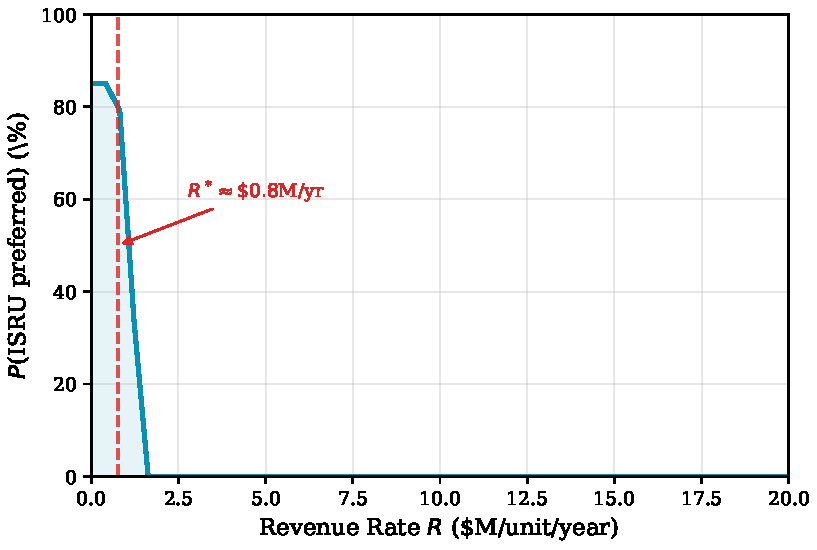
\includegraphics[width=\columnwidth]{fig-crossover-vs-revenue.pdf}
  \caption{Crossover point $N^*$ as a function of per-unit revenue rate $R$ (\$M/unit/yr) for asset lifetimes $L \in \{10, 20, 30\}$~yr ($r = 5\%$). Above the breakeven revenue $R^*$, the Earth pathway is preferred on a utility-maximizing basis despite higher cost.}
  \label{fig:crossover_vs_revenue}
\end{figure}

The breakeven revenue $R^* \approx \$0.94$M/unit/yr is insensitive to asset lifetime for $L \geq 10$~yr (because the ISRU delay $\bar{\delta} \approx 5.3$~yr is well below these lifetimes); it rises to \$1.84M/yr only at $L = 3$~yr, irrelevant for structural modules with expected lifetimes $>$20~yr. For block-deployed infrastructure (where units generate revenue only after the full constellation is operational), the per-unit opportunity cost computed here is an upper bound; the actual penalty depends on the block commissioning schedule.

At \$2M/yr revenue per unit (plausible for space solar power components), the opportunity cost exceeds the ISRU savings (\$22.7B), and the Earth pathway is preferred on a utility-maximizing basis despite being more expensive on a cost-minimizing basis. This finding underscores that the ISRU decision depends critically on whether the infrastructure is cost-driven (patient capital, no time pressure) or revenue-driven (commercial, time-to-market matters). Under a hybrid strategy (Earth-first for early units, ISRU for later units), the delay penalty applies only to post-transition units, so $R^*$ would be higher than the single-pathway value reported above; quantitative computation of the hybrid $R^*$ is deferred to future work. The opportunity cost penalty is maximized in a single-program scenario; if the ISRU infrastructure serves as a shared utility across multiple programs, the delay penalty is amortized and $R^*$ shifts upward, expanding the domain in which ISRU is preferred even for revenue-generating infrastructure.

\subsection{Implications for near-term space policy}

Several policy implications follow from the analysis:

\emph{ISRU technology demonstrations are high-value investments.} The dominance of the Earth manufacturing learning rate in the sensitivity analysis implies that the crossover depends critically on whether terrestrial production achieves the expected cost reductions. ISRU investment hedges against a future in which Earth manufacturing learning stalls---a scenario that would bring the crossover earlier by thousands of units. Current investments in lunar ISRU (Artemis program, CLPS payloads) and Mars ISRU (MOXIE follow-ons) should be evaluated not only for their direct mission benefits but for their contribution to de-risking the ISRU production pathway.

\emph{Launch cost reduction and ISRU investment are complementary.} Even at aggressive launch learning ($\mathrm{LR}_L = 0.90$), the crossover shifts by only $+$7\%, because the structural cost asymmetry persists regardless of launch cost level. Cheap launch is essential for deploying ISRU infrastructure itself.

\emph{The discount rate primarily affects crossover achievement probability, not crossover location.} The conditional median is stable at $\sim$4{,}200--5{,}700 units across $r \in [3\%, 8\%]$, while crossover achievement probability ranges from 79\% ($r = 3\%$) to 54\% ($r = 8\%$). This suggests that public-private partnership---combining patient public capital with commercial execution---is the natural financing structure for ISRU infrastructure.

\subsection{Decision framework}

Figure~\ref{fig:decision_tree} summarizes the practical decision logic for selecting between the Earth and ISRU pathways, integrating the key branching criteria identified in this analysis: production volume relative to $N^*$, discount rate regime, technical success probability, revenue generation rate, and vitamin fraction.

\begin{figure}[htbp]
  \centering
  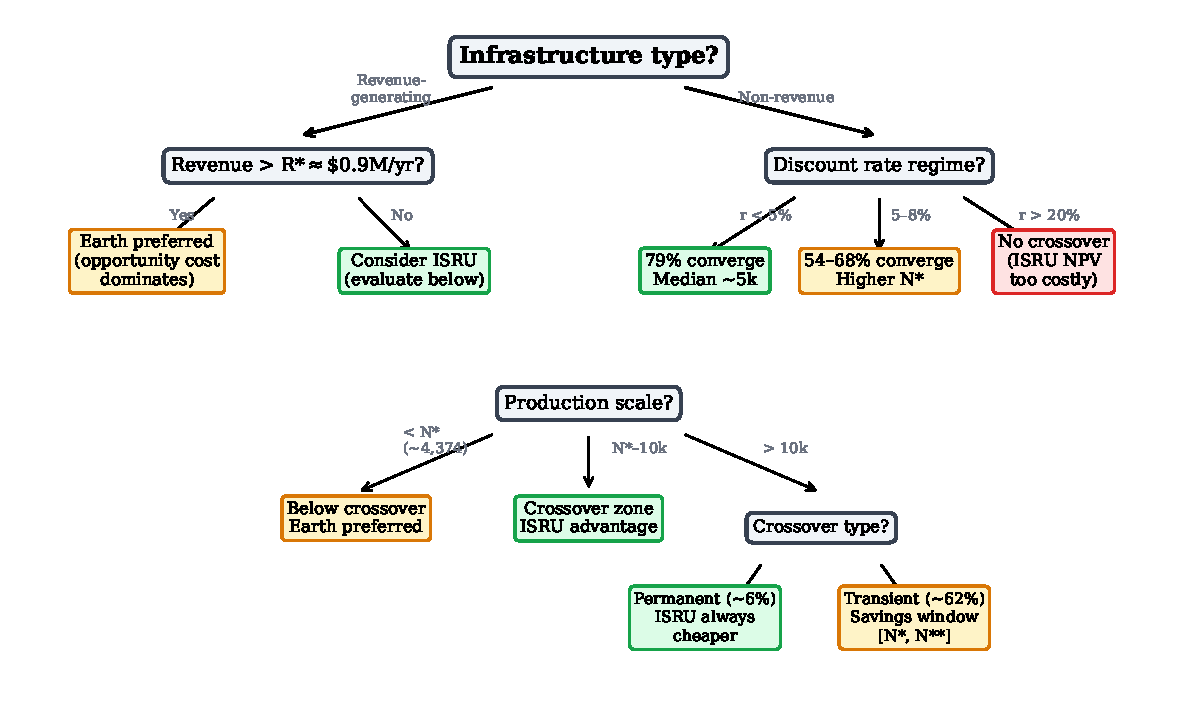
\includegraphics[width=\columnwidth]{fig-decision-tree.pdf}
  \caption{Decision framework for ISRU vs.\ Earth pathway selection, summarizing the key branching criteria identified in this analysis. Branch thresholds are model-derived: $R^*$ from Eq.~\ref{eq:revenue_breakeven}; discount rate regimes from MC crossover achievement rates (Table~\ref{tab:mc_summary}); $N^*$ from deterministic baseline (Table~\ref{tab:config}). Thresholds are illustrative; real decisions require updated data.}
  \label{fig:decision_tree}
\end{figure}

\subsection{Technology disruption scenarios}
\label{sec:tech_disruption}

The baseline model assumes static technology parameters over the multi-decade production horizon. To bound the sensitivity to technology step-changes, we test two deterministic disruption scenarios:

\paragraph{Scenario 1: Earth manufacturing cost halved at $n = 2{,}000$.} A breakthrough in automated manufacturing reduces $C_{\mathrm{mfg}}^{(1)}$ by 50\% for all units after $n = 2{,}000$ (e.g., fully automated additive manufacturing replacing labor-intensive assembly). Result: $N^* = 7{,}986$ (shift: $+$3{,}583, $+$81\% from baseline). The disruption significantly delays but does not prevent crossover.

\paragraph{Scenario 2: Launch cost drops to \$500/kg at $n = 2{,}000$.} A step-change in launch technology (e.g., next-generation reusable vehicle) halves the effective launch cost floor. Result: $N^* = 4{,}600$ (shift: $+$197, $+$4.5\% from baseline). The crossover is nearly unaffected because the structural manufacturing cost asymmetry---not launch cost---drives the result.

When the disruption occurs \emph{after} the crossover ($n = 5{,}000 > N^* = 4{,}403$), both scenarios produce zero shift, confirming that the crossover result is path-dependent on pre-crossover costs. The Scenario~1 result ($+$81\%) represents a worst case: even a 50\% step-change in Earth manufacturing cost, occurring before the crossover, delays it to ${\sim}8{,}000$~units---still within the MC interquartile range. Note that symmetric disruptions favoring the ISRU pathway (e.g., reduced $K$ or improved extraction efficiency) are already captured by the MC uncertainty ranges.

\subsection{Limitations and future work}

The dominant model parameters---LR$_E$ (PRCC $= -0.94$) and $K$ (PRCC $= +0.90$)---have been partially grounded: LR$_E$ is cross-checked against Iridium NEXT production data (implied $\mathrm{LR}_E \approx 0.85$, \S\ref{sec:sensitivity}), and the $K$ distribution is calibrated to Flyvbjerg's megaproject reference class \cite{flyvbjerg2014}. However, both lack bottom-up engineering calibration for the specific product class modeled; anchoring $K$ to a reference ISRU architecture with subsystem-level cost estimates would further strengthen the analysis.

\paragraph{ISRU pathway empirical grounding gap.} While the Earth pathway is cross-checked against Iridium NEXT production data (\S\ref{sec:sensitivity}), the ISRU pathway lacks an equivalent empirical anchor. No extraterrestrial manufacturing facility has operated at the scale modeled, and the ISRU learning rate ($\mathrm{LR}_I = 0.90$) relies entirely on terrestrial analogy. Three conservative modeling choices partially mitigate this gap: (1)~$\mathrm{LR}_I = 0.90$ is conservative relative to terrestrial additive manufacturing analogs (Table~\ref{tab:empirical_lr}), which achieve 0.85--0.92; (2)~the no-learning boundary test ($\mathrm{LR}_I = 1.0$) demonstrates that crossover is preserved even without any ISRU learning; and (3)~the pioneering phase test ($\gamma = 2$--$5\times$ for the first 100--1{,}000 units) directly models negative learning (cost increases during debugging). The symmetric learning plateau test (\S\ref{sec:sensitivity}) extends this by also testing learning moderation on the ISRU pathway after $n > n_{\mathrm{break}}$ units, confirming that the net effect of dual-pathway plateau is modest. Nevertheless, a direct cross-check against sub-process ISRU cost models (e.g., Sanders \& Larson propellant production \cite{sanders2015}) remains an important priority for future work.

The piecewise learning plateau model (\S\ref{sec:sensitivity}) addresses the Wright curve extrapolation concern but is itself a parametric approximation; micro-level learning models (e.g., Benkard \cite{benkard2000}) would provide more rigorous high-volume cost projections.

The model assumes a fixed unit design over the production horizon. This ``frozen design'' assumption is standard practice for commodity structural products (e.g., steel I-beams, concrete panels, satellite bus platforms), where the production tooling is optimized once and the design is held constant to maximize learning-curve benefits. For the ISRU pathway, frozen design is conservative: design improvements during production would reduce the mass penalty $\alpha$ and vitamin fraction $f_v$, favoring ISRU. For the Earth pathway, frozen design is mildly optimistic: disruptive manufacturing advances (e.g., large-format additive manufacturing) could reduce $C_{\mathrm{mfg}}^{(1)}$ by a step change not captured by the smooth Wright curve. In practice, both pathways will experience technology evolution: Earth manufacturing may benefit from advances in additive manufacturing and automation, while ISRU may benefit from improved extraction and refining processes. Two deterministic technology disruption scenarios are tested in \S\ref{sec:tech_disruption} (Earth cost halved at $n = 2{,}000$; launch cost dropped to \$500/kg at $n = 2{,}000$); extending this to stochastic disruptions with uncertain timing and magnitude remains future work. Similarly, at very large production scales the vitamin fraction may decline as ISRU capabilities mature, converting transient crossovers to permanent ones; modeling a dynamic $f_v(n)$ is deferred to future work.

Several methodological extensions are planned: (1)~accelerated failure time or Cox regression to handle right-censored non-converging observations more rigorously than conditional statistics; (2)~real options analysis incorporating stochastic $K$ and $t_0$ with abandonment optionality, which would better capture the value of staged ISRU commitment than the constant-rate NPV framework used here; (3)~multi-product modeling with shared ISRU infrastructure, which would shift the crossover earlier through capital amortization across product lines; and (4)~calibration against sub-process ISRU models (e.g., Sanders \& Larson propellant production \cite{sanders2015}) for specific ISRU product classes. The success probability framework (\S\ref{sec:success_probability}) assumes all-or-nothing failure; a two-stage decision tree with partial success and salvage value would lower $p_s^{\min}$ at all horizons.

%% ============================================================
\section{Conclusion}
\label{sec:conclusion}
%% ============================================================

For a program committing to 20{,}000 units, 42\% (95\% bootstrap CI: [41\%, 43\%]) of Monte Carlo scenarios at $r = 5\%$ fall within the ISRU savings window---the decision-relevant metric for finite-horizon programs. The raw crossover probability is ${\sim}$69\% (within $H = 40{,}000$ units), decomposed into ${\sim}$6\% permanent and ${\sim}$63\% transient, with a conditional median of $\sim$5{,}000~units. Rank-regression variance decomposition confirms that LR$_E$ and $K$ together explain ${\sim}$70\% of output variance, and over 30 robustness tests confirm crossover with no single test shifting it by more than 25\%. Three factors can prevent crossover: vitamin component costs above ${\sim}$\$50{,}000/kg, discount rates above ${\sim}$20\%, or low technical success probability ($p_s \lesssim 70\%$).

The ISRU decision is as much a financial structuring problem as a technological one: programs with patient capital find ISRU compelling at 2{,}000--4{,}400 units, while commercial hurdle rates prevent crossover. For revenue-generating infrastructure, the opportunity cost of ISRU's deployment delay may exceed the cost savings at revenue rates above ${\sim}$\$0.9M/unit/yr, suggesting the ISRU advantage is strongest for non-revenue infrastructure. Our analysis supports a hybrid strategy---Earth manufacturing for initial capability, ISRU for long-run cost advantage---with launch cost reduction and ISRU investment as complementary pursuits.

\section*{Code Availability}

The Python simulation code (\texttt{isru\_model.py}, \texttt{isru\_mc.py}, \texttt{generate\_isru\_figures.py}) and associated test suite are available at \url{https://github.com/project-dyson} under an open-source license. Results in this paper were generated from version~AF of the codebase (commit \texttt{PENDING}). A DOI-archived snapshot will be deposited upon acceptance.

%% ============================================================
%% References
%% ============================================================

\section*{Acknowledgments}

This research was conducted as part of Project Dyson, a non-profit open research initiative. The simulation code is available at \url{https://github.com/project-dyson}.

\section*{Conflicts of Interest}

The authors declare no competing interests. This research received no external funding.

\appendix
\section{Supplementary Sensitivity Tests}
\label{sec:appendix_sensitivity}

Table~\ref{tab:robustness_summary} summarizes sensitivity tests with individually small or moderate impact on the crossover. Detailed descriptions follow.

\begin{table}[htbp]
\centering
\caption{Summary of robustness tests (NPV, $r = 5\%$, baseline $N^* = 4{,}403$).}
\label{tab:robustness_summary}
\small
\begin{tabular}{@{}lrl@{}}
\toprule
Test & Max shift & Direction \\
\midrule
S-curve steepness ($k = 0.5$--$4.0$) & $\pm$5 & Negligible \\
Launch learning re-indexing ($\lambda = 0.5$--$2.0$) & $\pm$15 & Negligible \\
Rate-dependent learning (20--30\% threshold) & 0 & None \\
Piecewise construction schedule ($t_c = t_0 - 1$) & 0 & None \\
ISRU pre-purchase timing ($\tau = 0.5$--$1.0$~yr) & $+$18 & Delays \\
Earth mfg floor ($C_{\mathrm{mfg}}^{\mathrm{floor}} \leq \$3$M) & 0 & None \\
Fuel floor decomposition (fixed total) & $\pm$44 & Negligible \\
$K$--$\dot{n}$ correlation ($\rho = 0$ vs.\ $0.5$) & $-$185 & Earlier \\
Earth-side fixed costs ($K_E = \$1$--$10$B) & $-$1{,}187 & Earlier (favors ISRU) \\
Earth scaling penalty ($\gamma_E = 1.1$--$1.3$) & $-$301 to $-$720 & Earlier (favors ISRU) \\
Extended 6D copula ($K$--$t_0$, $K$--$A$, $K$--$C_{\mathrm{ops}}^{(1)}$) & $-$0.5~pp & Negligible \\
Asymmetric plateau (Earth continues, ISRU stalls) & $+$167 & Minor \\
\bottomrule
\end{tabular}
\end{table}

\paragraph{S-curve steepness.} Sweeping $k \in \{0.5, 1.0, 2.0, 3.0, 4.0\}$ shifts the crossover by $\pm$5~units; the crossover occurs well past the ramp-up phase.

\paragraph{Launch learning re-indexing.} Testing $\lambda \in \{0.5, 1.0, 2.0\}$ (co-manifest vs.\ dedicated launches) shifts the crossover by $\pm$15~units.

\paragraph{Fuel floor sensitivity.} Sweeping $p_{\mathrm{fuel}}$ from \$50 to \$400/kg with fixed total launch cost shifts the crossover by $\pm$44~units; the model is insensitive to the fuel-vs-operations split.

\paragraph{Rate-dependent learning.} A rate-dependent modifier freezing the learning curve below 20--30\% capacity has zero effect under baseline ramp-up ($k = 2.0$).

\paragraph{Piecewise construction schedule.} Enforcing $\dot{n}(t) = 0$ for $t < t_c = t_0 - 1$ produces no crossover shift; the exponentially small early production is negligible.

\paragraph{Cash-flow timing sensitivity.} Earth manufacturing lead times of 0.5--1.0~yr shift the crossover by $-$3.6\% to $-$6.6\% (earlier), confirming the pay-at-delivery simplification is slightly conservative.

\paragraph{ISRU operational pre-purchase timing.} Shifting ISRU operational costs earlier by 0.5--1.0~yr shifts the crossover by $+$0.3\% to $+$0.4\%, negligible compared to the Earth timing effect.

\paragraph{Earth-side fixed costs.} Adding Earth-side capital $K_E = \$1$--$10$B shifts the crossover by $-$129 to $-$1{,}187~units, uniformly favoring ISRU.

\paragraph{ISRU cost floor threshold (detail).} Crossover is achieved for all $C_{\mathrm{floor}}$ up to \$3.0M (the stochastic upper bound) and persists to \$10M ($N^* = 10{,}847$) via finite-horizon amortization (the permanent crossover threshold $C_{\mathrm{floor}} < \$1.67$M is derived in \S\ref{sec:cfloor_prodrate}).

\paragraph{Ongoing capital maintenance (detail).} Periodic maintenance at $\phi_K \cdot K$ every $\Delta t_K$ years adds a recurring cost stream:
\begin{equation}
  C_{\mathrm{maint}} = \sum_{j=1}^{\lfloor T/\Delta t_K \rfloor} \frac{\phi_K \cdot K}{(1+r)^{j \cdot \Delta t_K}},
\end{equation}
where $T = N/\dot{n}_{\max}$ is the program duration. With $\Delta t_K = 5$~yr: $\phi_K = 5\%$ shifts the crossover by $+$1{,}435; $\phi_K = 10\%$ by $+$3{,}215; $\phi_K = 15\%$ by $+$5{,}515. The crossover remains within the MC range for $\phi_K \leq 10\%$.

\paragraph{Earth manufacturing cost floor (detail).} To test whether the Wright learning curve overestimates cost reduction at high volumes (where Earth manufacturing may transition to commodity-like production with material-dominated costs), we sweep $C_{\mathrm{mfg}}^{\mathrm{floor}} \in \{0, \$2\text{M}, \$5\text{M}, \$10\text{M}\}$. The crossover is unaffected at all tested floor values up to \$3M ($N^* = 4{,}077$ throughout). This is because at the crossover volume ($\sim$4{,}400 units), the unfloored Earth mfg cost ($C_{\mathrm{mfg}}^{(1)} \cdot n^{b_E} \approx \$8$M) is already above even the highest floor tested. At $n = 10{,}000$: with no floor, Earth unit cost is \$10.0M; with $C_{\mathrm{mfg}}^{\mathrm{floor}} = \$10$M, it rises to \$11.4M. The floor would matter only for production volumes well beyond 10{,}000 units, where the learning curve would have driven mfg cost below the floor.

\paragraph{Capital--production rate correlation.} The baseline Monte Carlo correlates ISRU capital $K$ and production rate $\dot{n}_{\max}$ ($\rho_{K,\dot{n}} = 0.5$) via the extended Gaussian copula (\S\ref{sec:model}), reflecting that higher-capacity facilities require larger capital investment. This eliminates implausible corner cases (e.g., $K = \$100$B with $\dot{n}_{\max} = 250$ units/yr). As a sensitivity test, we run with $\rho_{K,\dot{n}} = 0$ (full independence): the convergence rate decreases from 79.4\% to 76.6\% and the conditional median moves from 5{,}800 to 5{,}615 ($-$185~units, $-$3\%). These results confirm that the correlation assumption is not a material driver of the conclusions.

\paragraph{Extended 6D copula.} The baseline 3D copula correlates only $(p_{\mathrm{launch}}, K, \dot{n}_{\max})$. To test whether plausible correlations among the remaining parameters materially affect results, we extend the copula to 6D, adding $\rho(K, t_0) = +0.4$ (larger facility $\to$ longer ramp-up), $\rho(K, A) = -0.3$ (larger facility $\to$ more downtime), and $\rho(K, C_{\mathrm{ops}}^{(1)}) = +0.3$ (larger facility $\to$ higher initial ops). All other new off-diagonals are zero; existing correlations are preserved. Table~\ref{tab:copula_6d} compares the results at $r = 5\%$.

\begin{table}[htbp]
\centering
\caption{Extended copula sensitivity: 3D (baseline) vs.\ 6D copula (10{,}000~runs, $r = 5\%$, $H = 40{,}000$, same seed).}
\label{tab:copula_6d}
\small
\begin{tabular}{@{}lrrr@{}}
\toprule
Copula & Conv.\ \% & Cond.\ median & Shift \\
\midrule
3D (baseline) & 69.0\% & 4{,}921 & --- \\
6D (extended) & 68.5\% & 4{,}701 & $-$0.5~pp \\
\bottomrule
\end{tabular}
\end{table}

The extended copula shifts convergence by $-$0.5~pp and the conditional median by $-$220~units ($-$4.5\%), confirming that correlations among the three additional parameters do not materially alter the headline results. The negative median shift arises because $\rho(K, A) < 0$ penalizes high-$K$ scenarios with lower availability, slightly reducing the number of marginally non-converging runs.

\paragraph{Asymmetric learning plateau.} The symmetric plateau test (\S\ref{sec:sensitivity}) assumes both pathways plateau simultaneously. A more adverse scenario for ISRU is one in which Earth learning continues unabated while ISRU learning stalls. With Earth damping $= 1.0$ (no plateau) and ISRU damping $= 0.3$ at $n_{\mathrm{break}} = 200$: $N^* = 4{,}541$ (shift: $+$167). With ISRU damping $= 0.5$ at $n_{\mathrm{break}} = 500$: $N^* = 4{,}455$ (shift: $+$81). Both worst-case asymmetric shifts are well below the $\mathrm{LR}_I = 1.0$ boundary test ($+$1{,}679), confirming that asymmetric plateau is not a decisive risk factor.

\paragraph{Pioneering phase (negative learning).} The baseline Wright curve assumes monotonically decreasing costs from unit~1. In practice, the first ISRU units may experience cost increases due to debugging, equipment failures, and process redesign. We test a two-phase model with cost multiplied by $\gamma \geq 1$ for the first $n_p$ units. At $\gamma = 2$, $n_p = 100$: $+$34 units ($+$0.8\%); $n_p = 500$: $+$136 ($+$3.1\%); $n_p = 1{,}000$: $+$246 ($+$5.6\%). At $\gamma = 5$, $n_p = 500$: $+$559 ($+$12.7\%); $n_p = 1{,}000$: $+$1{,}037 ($+$23.6\%). The $\mathrm{LR}_I = 1.0$ boundary test ($+$1{,}679 units) remains more conservative than any pioneering phase at $n_p \leq 500$.

\paragraph{Quality assurance and certification costs.} We add a QA cost $C_{\mathrm{QA}}^{(1)}$ declining with learning rate $\mathrm{LR}_{\mathrm{QA}}$. At $C_{\mathrm{QA}}^{(1)} = \$1$M, $\mathrm{LR}_{\mathrm{QA}} = 0.85$: $+$73 units ($+$1.7\%). At $C_{\mathrm{QA}}^{(1)} = \$3$M, $\mathrm{LR}_{\mathrm{QA}} = 0.90$: $+$421 units ($+$9.6\%). Even conservative QA assumptions shift the crossover by $<$10\%.

\paragraph{$K$ clip bound sensitivity (detail).}

\begin{table}[htbp]
\centering
\caption{$K$ clip upper bound sensitivity (10{,}000~runs, $r = 5\%$, $H = 40{,}000$). Raising the clip from \$200B to \$500B has negligible effect on convergence or conditional median.}
\label{tab:k_clip}
\small
\begin{tabular}{@{}rrrrr@{}}
\toprule
$K_{\max}$ clip & Conv.\ \% & Cond.\ median & $K$ P90 & $K$ P99 \\
\midrule
\$200B & 68.1\% & 4{,}976 & \$163B & \$200B \\
\$300B & 67.7\% & 4{,}931 & \$163B & \$300B \\
\$500B & 67.6\% & 4{,}930 & \$163B & \$344B \\
\bottomrule
\end{tabular}
\end{table}

\paragraph{Earth pathway cross-check (detail).} To cross-check the Earth cost model against real production data, we map it to the Iridium NEXT constellation. Thales Alenia Space manufactured 81~satellites (bus mass $\sim$860~kg each) under a contract valued at approximately \$2.1B. Setting $C_{\mathrm{mfg}}^{(1)} = \$80$M, the Wright curve at $\mathrm{LR}_E = 0.80$ predicts cumulative manufacturing cost of \$2.26B at $n = 81$, closely matching the contract value ($2.26/2.1 = 1.07\times$). Reverse-fitting to the \$2.1B total yields an implied $\mathrm{LR}_E \approx 0.79$, consistent with Wertz 2011 \cite{wertz2011} (0.83--0.88 for satellite buses, $n = 50$--$200$).

\paragraph{$n_0 \times \mathrm{LR}_E$ interaction (detail).}

\begin{table}[htbp]
\centering
\caption{$n_0 \times \mathrm{LR}_E$ interaction ($r = 5\%$). Each cell shows $N^*$; $>$40k indicates no crossover within 40{,}000~units.}
\label{tab:n0_lr_interaction}
\small
\begin{tabular}{@{}rrrrrr@{}}
\toprule
 & \multicolumn{4}{c}{$\mathrm{LR}_E$} \\
\cmidrule(l){2-5}
$n_0$ & 0.80 & 0.85 & 0.90 & 0.95 \\
\midrule
0   & 21{,}365 & 4{,}403 & 1{,}987 & 1{,}111 \\
50  & 25{,}051 & 4{,}600 & 2{,}050 & 1{,}130 \\
100 & 27{,}973 & 4{,}720 & 2{,}089 & 1{,}143 \\
200 & 35{,}249 & 4{,}907 & 2{,}149 & 1{,}162 \\
500 & $>$40k   & 5{,}309 & 2{,}276 & 1{,}201 \\
\bottomrule
\end{tabular}
\end{table}

\paragraph{Kaplan-Meier survival analysis (detail).}

\begin{table}[htbp]
\centering
\caption{Kaplan-Meier median vs.\ conditional median for the crossover distribution at three discount rates (10{,}000 MC runs, $H = 40{,}000$). The KM estimator accounts for right-censored observations; divergence quantifies the bias from ignoring censoring.}
\label{tab:kaplan_meier}
\small
\begin{tabular}{@{}rrrrr@{}}
\toprule
$r$ & Conv.\ \% & Cond.\ median & KM median & Divergence \\
\midrule
3\%  & 78.6\% & 5{,}654 & 8{,}112  & 43.5\% \\
5\%  & 68.1\% & 4{,}976 & 9{,}457  & 90.1\% \\
8\%  & 53.5\% & 4{,}218 & 16{,}147 & 282.9\% \\
\bottomrule
\end{tabular}
\end{table}

Divergence increases sharply with censoring: 44\% at $r = 3\%$, 283\% at $r = 8\%$.

\paragraph{Convergence as a function of planning horizon.} The choice of planning horizon $H = 40{,}000$ units is somewhat arbitrary. Figure~\ref{fig:convergence_curve} presents the empirical CDF $P(N^* \leq H)$ as a continuous function of $H$ for three discount rates, removing the dependence on any single horizon choice. At $H = 10{,}000$, convergence is 60\% ($r = 5\%$); at $H = 20{,}000$, 74\%; results plateau beyond $H \approx 30{,}000$ as marginal scenarios are exhausted. The figure provides a decision tool: a program planner can read off the probability of achieving crossover given their specific production horizon.

\begin{figure}[htbp]
  \centering
  
\includegraphics[width=\columnwidth]{fig-convergence-curve.pdf}
  \caption{Probability of achieving crossover $P(N^* \leq H)$ as a continuous function of planning horizon $H$, for three discount rates ($r = 3\%, 5\%, 8\%$). Based on 10{,}000 MC runs per rate. Vertical dashed lines mark $H = 10{,}000$ and $H = 20{,}000$.}
  \label{fig:convergence_curve}
\end{figure}

\paragraph{Bootstrap confidence intervals for savings window.} The savings window probabilities in Table~\ref{tab:savings_survival} are computed from 10{,}000 MC runs. To quantify sampling uncertainty, we construct 95\% bootstrap confidence intervals by resampling the converging runs 5{,}000 times with replacement, computing the savings window probability at each horizon for each resample, and reporting the 2.5th and 97.5th percentiles. The resulting CI widths ($\pm$1.0--1.2~pp) confirm that the 10{,}000-run ensemble provides adequate precision for the headline ``42\%'' figure (95\% CI: [41\%, 43\%]).

\section{Schedule and Model Details}
\label{sec:appendix_schedule}

\paragraph{Schedule model verification.} Substituting $n = 1$ into Eq.~\ref{eq:production_schedule} yields $t_{1,I} = t_0 + (1/k)\ln(2e^{k/\dot{n}_{\max}} - 1) \approx t_0$, confirming that the first unit is produced near the ramp-up midpoint, with $S(t_0) = 0.50$. The piecewise enforcement ($\dot{n} = 0$ for $t < t_c$) affects only the exponentially small tail before $t_c$; $N(t_c)$ is negligible (${\sim}10^{-3}$ units). The counting convention starts from $N(t_0) = 0$, not from facility groundbreaking.

\begin{table}[htbp]
\centering
\caption{Pathway-specific delivery schedules. The gap column shows the additional time ISRU requires relative to Earth delivery of the same unit number.}
\label{tab:production_schedule}
\small
\begin{tabular}{@{}rrrrr@{}}
\toprule
Unit $n$ & $t_{n,E}$ (yr) & $t_{n,I}$ (yr) & $S(t_{n,I})$ & Gap (yr) \\
\midrule
1      & 0.002 & 5.00  & 0.50 & $+$5.00 \\
10     & 0.02  & 5.04  & 0.52 & $+$5.02 \\
100    & 0.20  & 5.34  & 0.66 & $+$5.14 \\
500    & 1.00  & 6.31  & 0.93 & $+$5.31 \\
1{,}000  & 2.00  & 7.34  & 0.99 & $+$5.34 \\
5{,}000  & 10.00 & 15.35 & 1.00 & $+$5.35 \\
10{,}000 & 20.00 & 25.35 & 1.00 & $+$5.35 \\
\bottomrule
\end{tabular}
\end{table}

\paragraph{Deterministic vs.\ MC capital estimates.} The deterministic baseline uses $K = \$50$B (the modal estimate for a first-of-kind vertically integrated ISRU facility), while the MC median is $K = \$65$B. This difference arises because the log-normal distribution is right-skewed: the mode of $\mathrm{LN}(\mu_{\ln}, \sigma_{\ln})$ is $e^{\mu_{\ln} - \sigma_{\ln}^2} = \$46$B, while the median is $e^{\mu_{\ln}} = \$65$B. The deterministic \$50B lies between these values; the MC correctly propagates the full distribution.

\section{Throughput Analysis Details}
\label{sec:appendix_throughput}

At 500 Starship launches per year at 100{,}000~kg payload capacity, Earth can deliver 50{,}000~tonnes/year. A $10^5$-unit program (185{,}000~tonnes) would require $\sim$3.7~years of dedicated capacity; a $10^6$-unit program would require 18{,}500~launches over 37~years. Total global launch mass in 2023 was $\sim$1{,}200~tonnes \cite{jones2022}. We tested Earth delivery rate caps of 2{,}000--27{,}000~units/yr ($\sim$37--500 Starship-equivalent launches/yr); at all caps the crossover is unchanged from baseline because the production rate (500~units/yr) is well below even the most conservative cap. Table~\ref{tab:demand_scenarios} maps crossover volumes to illustrative architectures.

\begin{table}[htbp]
\centering
\caption{Illustrative demand scenarios for 1{,}850~kg structural modules. Mass estimates are order-of-magnitude \cite{jones2022,oneill1976}.}
\label{tab:demand_scenarios}
\small
\begin{tabular}{@{}lrrrl@{}}
\toprule
Architecture & Mass & Units & Timeline & Crossover? \\
\midrule
1~GW SPS demo$^\star$ & 5{,}000~t & 2{,}700 & 10--15~yr & Below $N^*$ \\
10~GW SPS constellation$^\star$ & 50{,}000~t & 27{,}000 & 20--30~yr & Above $N^*$ \\
O'Neill cylinder & 500{,}000~t & 270{,}000 & 30--50~yr & Far above $N^*$ \\
\bottomrule
\multicolumn{5}{@{}l}{\footnotesize $^\star$Revenue-qualified: SPS structural modules may generate $>\$0.9$M/unit/yr, in which} \\
\multicolumn{5}{@{}l}{\footnotesize case the Earth pathway is preferred on a utility-maximizing basis (\S\ref{sec:discussion}).}
\end{tabular}
\end{table}

\section{Parameter Justification Details}
\label{sec:appendix_params}

\emph{First-unit ISRU operational cost $C_{\mathrm{ops}}^{(1)} = \$5$M.} Sintering or melting regolith requires approximately 1{,}000~kWh per tonne of processed material \cite{cilliers2023}; a 1{,}850~kg unit requiring $\sim$5~tonnes of raw feedstock (at $\sim$37\% structural yield) consumes $\sim$5{,}000~kWh. At lunar surface power costs of $\sim$\$100--200/kWh \cite{sanders2015,lsic2021}, the energy component is \$0.5--1.0M. Adding equipment wear, consumable replacement, and remote operations overhead yields $\sim$\$5M under immature conditions.

\emph{ISRU capital $K = \$50$B.} This covers the complete chain: prospecting, extraction, processing, fabrication, and quality control, deployed without an existing supply chain. For context, ISS lifecycle cost is $\sim$\$150B; Artemis is budgeted at $\sim$\$93B. The capital cost per unit of annual throughput ($K/\dot{n}_{\max} = \$100$M per unit/year) is comparable to offshore oil platforms (\$5--15B, single-commodity) and nuclear plants (\$10--25B), adjusted for the uniquely challenging operational environment.

\paragraph{$K$ subsystem decomposition.} A rough breakdown of the \$50B baseline:
\begin{itemize}
  \item \emph{Power system} (${\sim}$\$8B): 50~MW nuclear/solar at ${\sim}$\$160M/MW.
  \item \emph{Mining \& processing} (${\sim}$\$12B): excavation, beneficiation, smelting.
  \item \emph{Fabrication facility} (${\sim}$\$10B): additive manufacturing + assembly.
  \item \emph{Transport \& logistics} (${\sim}$\$5B): landing pads, propellant depot, tugs.
  \item \emph{Habitat \& ops support} (${\sim}$\$5B): crew/teleops infrastructure.
  \item \emph{Integration, margin, delivery} (${\sim}$\$10B): 20\% margin + launch to surface at ${\sim}$\$5{,}000/kg for ${\sim}$500~t.
\end{itemize}
These figures are order-of-magnitude estimates for context; the Monte Carlo samples $K$ from the full log-normal distribution rather than decomposing it into subsystems.

\paragraph{$K$-median sensitivity.} To assess convergence behavior across a range of capital cost assumptions, Table~\ref{tab:k_median_sweep} reports 10{,}000-run MC results at $r = 5\%$ for $K$ medians from \$50B to \$150B (log-normal shape preserved, $\sigma_{\ln} = 0.70$, median rescaled). At the baseline median (\$65B), the convergence rate is 69\% and the conditional median is $\sim$4{,}900; doubling the median to \$150B reduces convergence to 27\% and roughly doubles the conditional median, confirming that $K$ is the dominant driver of crossover probability.

\begin{table}[htbp]
\centering
\caption{$K$-median sensitivity (10{,}000~MC runs, $r = 5\%$, $H = 40{,}000$, $\sigma_{\ln} = 0.70$). The $K = \$65$B row matches the baseline MC.}
\label{tab:k_median_sweep}
\small
\begin{tabular}{@{}rrrrl@{}}
\toprule
$K$ median & Det.\ $N^*$ & Conv.\ \% & Cond.\ median & Cond.\ IQR \\
\midrule
\$50B  & 4{,}374  & 80.1\% & 3{,}891  & [1{,}937, 7{,}946] \\
\$65B  & 6{,}952  & 69.0\% & 4{,}921  & [2{,}523, 9{,}851] \\
\$75B  & 9{,}328  & 61.9\% & 5{,}564  & [2{,}896, 10{,}810] \\
\$100B & 22{,}993 & 47.1\% & 7{,}020  & [3{,}728, 12{,}558] \\
\$150B & $>$40k   & 26.7\% & 8{,}698  & [5{,}104, 15{,}039] \\
\bottomrule
\end{tabular}
\end{table}

\emph{Earth-sourced component fraction (vitamin model).} The vitamin fraction model (Eq.~\ref{eq:vitamin} in \S\ref{sec:vitamin}) modifies the ISRU operational cost to account for components that cannot be ISRU-sourced. Sensitivity tests span $f_v \in \{0, 0.05, 0.10, 0.15, 0.20\}$ and $c_{\mathrm{vit}} \in \{\$5{,}000, \$10{,}000, \$50{,}000\}$/kg.

\paragraph{Cost basis normalization detail.} The $U[\$100, \$400]$ propellant floor range is grounded in a bottom-up decomposition:
\begin{enumerate}
  \item \emph{Propellant to LEO}: LOX at $\sim$\$0.20/kg and CH$_4$ at $\sim$\$0.40/kg, with a propellant-to-payload mass ratio of $\sim$25--37:1 for Starship-class vehicles, yields $\sim$\$5--8/kg of payload.
  \item \emph{LEO-to-GEO transfer}: $\Delta v \approx 3.9$--$4.2$~km/s; a chemical tug costs $\sim$\$80--120/kg transferred, or $\sim$\$30--60/kg via solar electric propulsion.
  \item \emph{Ground operations}: Pad turnaround, range fees, and GSE amortization at high cadence ($>$50~flights/yr) yield $\sim$\$20--50/kg.
\end{enumerate}
Summing yields $\sim$\$105--178/kg to GEO.

\begin{table}[htbp]
\centering
\caption{Representative vitamin BOM for a 1{,}850~kg structural module. Components marked $^\dag$ are Earth-sourced in the baseline but potentially ISRU-sourced at maturity; only the irreducible mechanical 5\% ($f_v = 0.05$) enters the cost model. Sensors/wiring (3\%) are not included in $f_v$ because they are separately accounted for in integration overhead; if included, $f_v$ would rise to $\sim$0.08 and the crossover would shift by $\sim$$+$200~units (\S\ref{sec:sensitivity}).}
\label{tab:vitamin_bom}
\small
\begin{tabular}{@{}llrrl@{}}
\toprule
Component & Source & Mass \% & Mass (kg) & Note \\
\midrule
Al structure      & ISRU   & 85\% & 1{,}573 & Regolith-derived alloy \\
Ti fasteners      & Earth  &  5\% &    93   & Irreducible vitamin ($f_v$) \\
Thermal coatings  & Earth$^\dag$ &  4\% &    74   & Potentially ISRU at maturity \\
Sensors/wiring    & Earth  &  3\% &    56   & Rad-hard electronics$^\ddag$ \\
Seals/gaskets     & Earth$^\dag$ &  3\% &    56   & Polymer, potentially ISRU \\
\midrule
\textbf{Total}    &        & 100\% & 1{,}850 & \\
\quad Irreducible vitamin ($f_v = 0.05$) & & 5\% & 93 & Modeled fraction \\
\bottomrule
\multicolumn{5}{@{}l}{\footnotesize $^\dag$Potentially ISRU-sourced at high technology maturity; modeled as Earth-sourced in baseline.} \\
\multicolumn{5}{@{}l}{\footnotesize $^\ddag$Not included in $f_v = 0.05$; accounted for separately in integration overhead.}
\end{tabular}
\end{table}

\begin{table}[htbp]
\centering
\caption{Active model equations in baseline MC vs.\ sensitivity variants. ``Baseline MC'' is the configuration used for the 10{,}000-run ensemble at each discount rate; sensitivity variants activate or vary additional features one at a time.}
\label{tab:config}
\small
\begin{tabular}{@{}lcc@{}}
\toprule
Component & Baseline MC & Sensitivity variants \\
\midrule
Earth mfg: two-component (Eq.~\ref{eq:earth_mfg}) & \checkmark & --- \\
Earth mfg floor (Eq.~\ref{eq:earth_mfg_floor}) & off ($C_{\mathrm{mfg}}^{\mathrm{floor}}=0$) & sweep \$2--10M \\
Launch learning (Eq.~\ref{eq:earth_launch_learn}) & \checkmark ($\mathrm{LR}_L=0.97$) & sweep 0.90--1.00 \\
Vitamin fraction (Eq.~\ref{eq:vitamin}) & \checkmark ($f_v=0.05$) & sweep 0--0.20 \\
ISRU pioneering phase & off ($\gamma=1$) & $\gamma=2$--$5$, $n_p=100$--$1{,}000$ \\
ISRU QA cost & off ($C_{\mathrm{QA}}^{(1)}=0$) & \$1--3M \\
Piecewise ISRU schedule & \checkmark ($t_c = t_0-1$) & --- \\
Earth ramp-up & off (instant start) & $t_{0,E}=1$--$2$~yr \\
ISRU availability & \checkmark ($A \sim U[0.70, 0.95]$) & --- \\
Learning plateau (Earth) & off & $n_{\mathrm{break}}=200$--$2{,}000$, $\eta=0.3$--$0.7$ \\
Learning plateau (ISRU) & off & $n_{\mathrm{break}}=200$--$1{,}000$, $\eta=0.5$ \\
$\sigma_{\ln}$ sensitivity & 0.70 & 1.0, 1.3 \\
Earth scaling penalty & off ($\gamma_E = 1$) & $\gamma_E = 1.1$--$1.3$, $n_{\mathrm{scale}} = 2{,}000$ \\
Transport duration $\tau_{\mathrm{trans}}$ & \checkmark (0.5~yr) & sweep 0.25--2.0~yr \\
\bottomrule
\end{tabular}
\end{table}

\begin{table}[htbp]
\centering
\caption{Empirical learning rates from analogous production programs. Our ranges $\mathrm{LR}_E \sim \mathcal{N}(0.85, 0.03)$ [0.75, 0.95] and $\mathrm{LR}_I \sim \mathcal{N}(0.90, 0.03)$ [0.80, 0.98] encompass these empirical values.}
\label{tab:empirical_lr}
\small
\begin{tabular}{@{}llrl@{}}
\toprule
Program class & LR range & $n$ range & Source \\
\midrule
Satellite buses          & 0.83--0.88 & 50--200    & Wertz 2011 \cite{wertz2011} \\
Solar arrays             & 0.80--0.85 & 100--1{,}000 & Nagy et al.\ 2013 \cite{nagy2013} \\
Aircraft structures      & 0.80--0.85 & 500+       & Argote \& Epple 1990 \cite{argote1990} \\
Metal additive mfg.      & 0.85--0.92 & 10--100    & Baumers et al.\ 2016 \cite{baumers2016} \\
\bottomrule
\end{tabular}
\end{table}

\emph{Additional parameter notes.} Mass penalty $\alpha \sim U[1.0, 2.0]$ captures additional feedstock required for structural equivalence. Availability $A \sim U[0.70, 0.95]$ accounts for equipment failures and limited maintenance access. Transport cost $p_{\mathrm{transport}} \sim U[\$50, \$300]$/kg covers lunar surface-to-GEO delivery \cite{ishimatsu2016}. Production rate $\dot{n}_{\max} = 500$~units/year, sampled $U[250, 750]$, requires $\sim$5{,}000--10{,}000~tonnes/year of raw regolith, within proposed ISRU facility scales \cite{sanders2015}. Ricardian rent is not a concern: lunar regolith is abundant (${\sim}10^{15}$~tonnes in the top 5~m) and compositionally homogeneous at the scales modeled.

\section{Assumptions and Limitations}
\label{sec:appendix_assumptions}

Key simplifying assumptions: (1)~fixed unit mass (no design evolution); (2)~quality parity between pathways (optimistic for early ISRU); (3)~static production environment (no disruptive innovations); (4)~single product type (multi-product would shift crossover earlier); (5)~constant real discount rate (risk-adjusted rates differ between pathways in practice); (6)~Earth production capacity assumed available from program start (tested in Earth ramp-up robustness check). The phased capital model does not couple deployment timing to production schedule onset; this coupling is left for future work.

\begin{thebibliography}{99}

\bibitem{andrews2015}
D.~Andrews, K.~Bonner, A.~Butterworth, H.~Calber, B.~Craddock, S.~Diber, et~al.,
\newblock Defining a successful commercial asteroid mining program,
\newblock Acta Astronautica 108 (2015) 106--118.

\bibitem{argote1990}
L.~Argote, D.~Epple,
\newblock Learning curves in manufacturing,
\newblock Science 247~(4945) (1990) 920--924.

\bibitem{arrow2014}
K.~J.~Arrow, M.~L.~Cropper, C.~Gollier, B.~Groom, G.~M.~Heal, R.~G.~Newell, et~al.,
\newblock Should governments use a declining discount rate in project analysis?,
\newblock Review of Environmental Economics and Policy 8~(2) (2014) 145--163.

\bibitem{baumers2016}
M.~Baumers, P.~Dickens, C.~Tuck, R.~Hague,
\newblock The cost of additive manufacturing: Machine productivity, economies of scale and technology-push,
\newblock Technological Forecasting and Social Change 102 (2016) 193--201.

\bibitem{benkard2000}
C.~L.~Benkard,
\newblock Learning and forgetting: The dynamics of aircraft production,
\newblock American Economic Review 90~(4) (2000) 1034--1054.

\bibitem{cesaretti2014}
G.~Cesaretti, E.~Dini, X.~De~Kestelier, V.~Colla, L.~Pambaguian,
\newblock Building components for an outpost on the lunar soil by means of a novel 3D printing technology,
\newblock Acta Astronautica 93 (2014) 430--450.

\bibitem{cilliers2023}
J.~Cilliers, A.~Rasera, S.~Hadler,
\newblock Mineralogical and chemical processing of lunar regolith for ISRU,
\newblock Minerals Engineering 194 (2023) 108023.

\bibitem{crawford2015}
I.~A.~Crawford,
\newblock Lunar resources: A review,
\newblock Progress in Physical Geography 39~(2) (2015) 137--167.

\bibitem{deweck2004}
O.~L.~de~Weck, R.~de~Neufville, M.~Chaize,
\newblock Staged deployment of communications satellite constellations in low Earth orbit,
\newblock Journal of Aerospace Computing, Information, and Communication 1~(3) (2004) 119--136.

\bibitem{dixit1994}
A.~K.~Dixit, R.~S.~Pindyck,
\newblock Investment Under Uncertainty,
\newblock Princeton University Press, Princeton, NJ, 1994.

\bibitem{dutton1984}
J.~M.~Dutton, A.~Thomas,
\newblock Treating progress functions as a managerial opportunity,
\newblock Academy of Management Review 9~(2) (1984) 235--247.

\bibitem{flyvbjerg2014}
B.~Flyvbjerg,
\newblock What you should know about megaprojects and why: An overview,
\newblock Project Management Journal 45~(2) (2014) 6--19.

\bibitem{flyvbjerg2017}
B.~Flyvbjerg (Ed.),
\newblock The Oxford Handbook of Megaproject Management,
\newblock Oxford University Press, Oxford, 2017.

\bibitem{kavlak2018}
G.~Kavlak, J.~McNerney, J.~E.~Trancik,
\newblock Evaluating the causes of cost reduction in photovoltaic modules,
\newblock Energy Policy 123 (2018) 700--710.

\bibitem{elvis2012}
M.~Elvis,
\newblock Let's mine asteroids---for science and profit,
\newblock Nature 485 (2012) 549.

\bibitem{hecht2021}
M.~Hecht, J.~Hoffman, D.~Rapp, et~al.,
\newblock Mars Oxygen ISRU Experiment (MOXIE),
\newblock Space Science Reviews 217 (2021) 9.

\bibitem{ishimatsu2016}
T.~Ishimatsu, O.~L.~de~Weck, J.~A.~Hoffman, Y.~Ohkami, R.~Shishko,
\newblock Generalized multicommodity network flow model for the Earth--Moon--Mars logistics system,
\newblock Journal of Spacecraft and Rockets 53~(1) (2016) 25--38.

\bibitem{kaplan1958}
E.~L.~Kaplan, P.~Meier,
\newblock Nonparametric estimation from incomplete observations,
\newblock Journal of the American Statistical Association 53~(282) (1958) 457--481.

\bibitem{jones2018}
H.~W.~Jones,
\newblock The recent large reduction in space launch cost,
\newblock in: 48th International Conference on Environmental Systems, ICES-2018-81, 2018.

\bibitem{jones2020}
H.~W.~Jones,
\newblock The cost of space launch: History and outlook,
\newblock in: 50th International Conference on Environmental Systems, ICES-2020-415, 2020.

\bibitem{jones2022}
H.~W.~Jones,
\newblock The cost and weight of space launch for space solar power,
\newblock in: 51st International Conference on Environmental Systems, ICES-2022-164, 2022.

\bibitem{kornuta2019}
D.~Kornuta, A.~Abbud-Madrid, J.~Atkinson, et~al.,
\newblock Commercial lunar propellant architecture: A collaborative study of lunar propellant production,
\newblock REACH 13 (2019) 100026.

\bibitem{lsic2021}
Lunar Surface Innovation Consortium,
\newblock Lunar ISRU Technology Roadmap,
\newblock Johns Hopkins Applied Physics Laboratory, 2021.

\bibitem{metzger2013}
P.~T.~Metzger, A.~Muscatello, R.~P.~Mueller, J.~Mantovani,
\newblock Affordable, rapid bootstrapping of the space industry and solar system civilization,
\newblock Journal of Aerospace Engineering 26~(1) (2013) 18--29.

\bibitem{nagy2013}
B.~Nagy, J.~D.~Farmer, Q.~M.~Bui, J.~E.~Trancik,
\newblock Statistical basis for predicting technological progress,
\newblock PLoS ONE 8~(2) (2013) e52669.

\bibitem{nasa2015handbook}
NASA,
\newblock NASA Cost Estimating Handbook, Version 4.0,
\newblock NASA Office of the Chief Financial Officer, Washington, DC, 2015.

\bibitem{oneill1974}
G.~K.~O'Neill,
\newblock The colonization of space,
\newblock Physics Today 27~(9) (1974) 32--40.

\bibitem{oneill1976}
G.~K.~O'Neill,
\newblock The High Frontier: Human Colonies in Space,
\newblock William Morrow, New York, 1976.

\bibitem{saleh2003}
J.~H.~Saleh, D.~E.~Hastings, D.~J.~Newman,
\newblock Flexibility in system design and implications for aerospace systems,
\newblock Acta Astronautica 53~(12) (2003) 927--944.

\bibitem{sanders2015}
G.~B.~Sanders, W.~E.~Larson,
\newblock Progress made in lunar in situ resource utilization under NASA's Exploration Technology and Development Program,
\newblock Journal of Aerospace Engineering 28~(1) (2015) 04014075.

\bibitem{sonter1997}
M.~J.~Sonter,
\newblock The technical and economic feasibility of mining the near-Earth asteroids,
\newblock Acta Astronautica 41~(4--10) (1997) 637--647.

\bibitem{sowers2021}
G.~F.~Sowers,
\newblock The business case for lunar ice mining,
\newblock New Space 9~(2) (2021) 77--94.

\bibitem{sowers2023}
G.~F.~Sowers,
\newblock A cislunar economic framework,
\newblock New Space 11~(1) (2023) 5--18.

\bibitem{thompson2012}
P.~Thompson,
\newblock The relationship between unit cost and cumulative quantity and the evidence for organizational learning-by-doing,
\newblock Journal of Economic Perspectives 26~(3) (2012) 203--224.

\bibitem{werkheiser2015}
N.~Werkheiser, J.~Dunn, M.~Snyder, J.~Edmunson, K.~Cooper, M.~Johnston,
\newblock 3D printing in zero-G ISS technology demonstration,
\newblock in: AIAA SPACE 2015, AIAA-2015-4585, 2015.

\bibitem{wertz2011}
J.~R.~Wertz, D.~F.~Everett, J.~J.~Puschell (Eds.),
\newblock Space Mission Engineering: The New SMAD,
\newblock Microcosm Press, Hawthorne, CA, 2011.

\bibitem{wright1936}
T.~P.~Wright,
\newblock Factors affecting the cost of airplanes,
\newblock Journal of the Aeronautical Sciences 3~(4) (1936) 122--128.

\bibitem{zapata2019}
E.~Zapata,
\newblock An assessment of cost improvements in the NASA COTS/CRS program and implications for future NASA missions,
\newblock in: AIAA SPACE and Astronautics Forum, AIAA-2019-4268, 2019.

\bibitem{zubrin1996}
R.~Zubrin, R.~Wagner,
\newblock The Case for Mars: The Plan to Settle the Red Planet and Why We Must,
\newblock Free Press, New York, 1996.

\end{thebibliography}

\end{document}
